\chapter{Výběr komponent/zařízení}

Na obrázku \ref{fig:otopna-soustava-a-elektronika-rez-domu} je nákres otopné soustavy včetně jednotlivých zařízení pro ovládání této soustavy. Vzhledem k teoretické části, kdy popisuji princip zónové regulace vytápění, tak v samotné realizaci je pouze regulace vytápění na základě prostorové teploty z lokálních termostatů umístěných na chodbách. Nastíním vývoj realizace nástěnných snímačů prostorové teploty a software pro zónovou regulaci. Nyní popíši jednotlivá vybraná či navržená zařízení z~nákresu. 

\newpage

\begin{figure}[H]
    \centering
    \def\svgwidth{\columnwidth}
    \input{images/svg/otopna-soustava-a-elektronika-rez-domu.pdf_tex}
    \caption{Otopná soustava v domě včetně elektroniky pro řízení.}
    \label{fig:otopna-soustava-a-elektronika-rez-domu}
\end{figure}


\section{Centrální jednotka Raspberry Pi}
Pro centrální řídicí jednotku jsem vybral jednodeskový počítač Raspberry Pi model 4. Důvodem pro vybraní byla přímá podpora HA, velká uživatelská základna, která toto zařízení používá (nejen s HA, ale i s jiným softwarem), nízká a relativně vysoký výkon. V neposlední řadě na pozadí HA běží linuxová distribuce, takže ovládání je stejné jak při použití běžných desktopových verzí. Přehled specifikace zařízení je v tabulce \ref{tab:prehled-vybaveni-raspberry-pi-4-model-b}. Samotné Raspberry Pi je na obrázku \ref{fig:raspberry-pi-4-model-b}. Samozřejmě může vzniknout úvaha nad odolností tohoto zařízení např. vůči vnějšímu rušení, samotného rušení zařízení apod. Co se týče nasazení takového zařízení, většinou výrobci uvádějí že se jedná o~vývojové zařízení, které není určeno do koncového zařízení nebo případně splňují  základní certifikace ochrany. Průmyslovou certifikaci nesplňují nebo se na trhu nacházejí zařízení, které se průmyslovou aplikací chlubí (zde je nutné důkladně pročíst všechnu technickou dokumentaci), pak dále skutečně stojí za zvážení o jakou certifikaci se jedná, v jaké části průmyslu lze toto zařízení nasadit, ale i tak to může být dost velký risk. Ve většině případů je však nutné provést hardwarovou úpravu pro vysokou odolnost proti rušení, robustnost běžícího real time systému, RTC, typ paměti pro ukládání dat (typ média), životnost, technická podpora a mnohé další. V domácích podmínkách nejsou nutné všechny požadavky jako v průmyslu, nicméně je nutné minimálně hledět na ESD ochranu připojených periferií především u sběrnic, které jsou na delší vzdálenosti a způsob ukládání dat z pohledu životnosti paměťového média. Pro ESD ochranu jak samotného Raspberry Pi, tak i koncových zařízení je nutné zapojit mezi kabely sběrnice a zařízení ESD ochrany (takové ochrany jsou navrženy a popsány níže). SD kartu pro ukládání a běh samotného systému je vhodné změnit za médium s vetší životností, lze využít například domácí NAS a data ukládat do databáze, SD kartu používat pouze pro systém či USB flash disk. Případně zajistit postup s předpřipravenou zálohou pro obnovu nefunkčního systému apod. 

\begin{center}
\begin{table}[H]
\begin{tabular}{|c||c|}
\hline
\thead{Procesor} &  
\makecell{Broadcom BCM2711 \\ 
quad-core Cortex-A72 (ARM v8)
64-bit, 1,5 GHz} \\ 
\hline
\thead{RAM} & 4 GB LPDDR4 \\ 
\hline
\thead{Konektivita} & 
\makecell{2,4 GHz a 5.0 GHz IEEE 802.11b/g/n/ac \\
LAN, Bluetooth 5.0, BLE \\
Gigabit Ethernet \\
2 × USB 3.0 ports \\
2 × USB 2.0 ports} \\
\hline
\thead{GPIO} & 2 × 20 pinový header \\ 
\hline
\thead{Video a zvuk} & 
\makecell{
2 × micro HDMI porty \\
 MIPI DSI displejový port \\
 MIPI CSI kamerový port \\
čtyřpólový stereo audio a kompozitní video port} \\ 
\hline
\thead{Podpora SD karty} & Micro SD slot (pro systém a data) \\ 
\hline
\thead{Napájení} & 
\makecell{
5 V DC přes USB-C konektor (minimum 3 A) \\
5 V DC přes GPIO header \\
(minimum 3 A, bez vstupních ochran)} \\ 
\hline
\end{tabular}
\caption[Přehled vybavení Raspberry Pi 4 modelu B.]{Přehled vybavení Raspberry Pi 4 modelu B \cite{raspberry-pi-4-model-b-specifikace}.}
\label{tab:prehled-vybaveni-raspberry-pi-4-model-b} 
\end{table}
\end{center}


\begin{figure}[H]
    \centering
    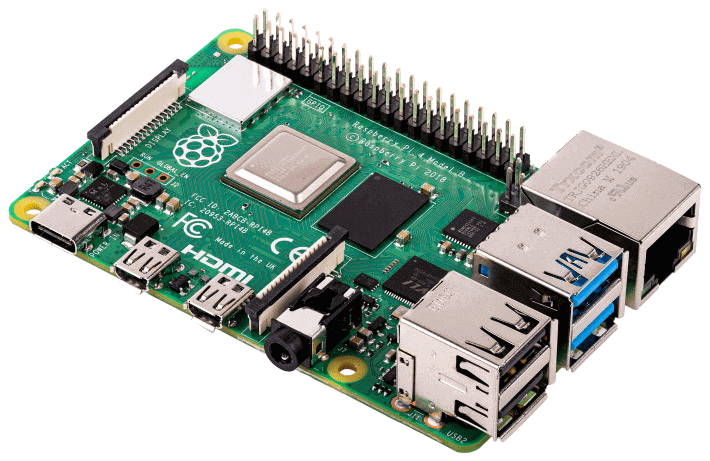
\includegraphics[width=\textwidth]{images/raspberry-pi-4-model-b.png}
    \caption[Raspberry Pi 4 model B.]{Raspberry Pi 4 model B. Upraveno z \cite{raspberry-pi-4-model-b}.}
    \label{fig:raspberry-pi-4-model-b}
\end{figure}

\section{Teplotní senzory}
\subsubsection{Teplotní senzory pro krby}
\label{sec:teplotni-senzory-pro-krby}
Pro snímání teploty z kouřovodů u krbů slouží termočlánek typu K od výrobce Guenther. Teplotní rozsah je od -100 °C do 400 °C, takže je dostatečná teplotní rezerva. Průměr kovové ochranné trubičky je 4 mm s délkou 60 mm. Přívodní kabel je dlouhý 3 m se skelným opletením. Termočlánek je zobrazen na obrázku \ref{fig:termoclanek-72-21301041-k}.

\begin{figure}[H]
    \centering
    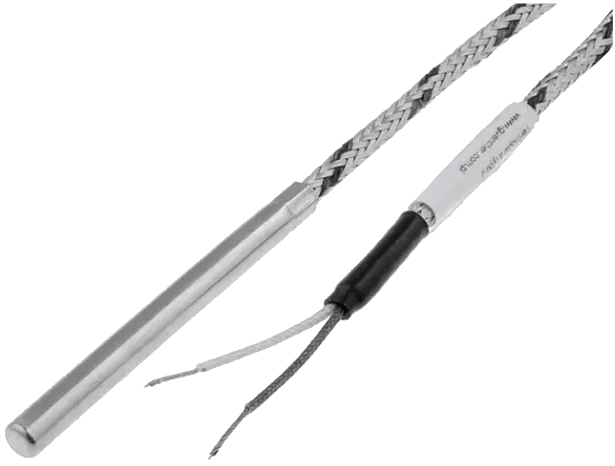
\includegraphics[width=0.5\textwidth]{images/termoclanek-72-21301041-k.png}
    \caption[Termočlánek 72-21301041 typu K.]{Termočlánek 72-21301041 typu K \cite{termoclanek-k}.}
    \label{fig:termoclanek-72-21301041-k}
\end{figure}

\subsubsection{Teplotní senzory na 1-Wire sběrnici}
Pro snímání teplot z centrálního zásobníku otopné vody, venkovní teploty a~prostorových teplot z jednotlivých místností slouží teplotní senzor DS18B20 od výrobce Maxim. Umožňuje měřit
v teplotním rozsahu od -+55 °C do +125~°C. V rozsahu od -10 °C do +85 °C měří s přesností ±0,5 °C. Senzor umožňuje měřit teplotu s přesností 12 bitů. Pro komunikaci využívá 1-Wire sběrnici (způsob komunikace je popsán v \ref{sec:1-wire-sbernice} v části 1-Wire sběrnice). Ve svém konkrétním řešením využívám senzory v pouzdře TO-92 pro nástěnné teplotní snímače prostorové teploty, pro centrální zásobník otopné vody a~venkovní teplotu je senzor zapouzdřen do ochranného pouzdra.


\section{\acrshort{dps} se vstupy/výstupu pro Raspberry Pi}
\label{sec:dps-se-vstupy-vystupy-pro-raspberry-pi}

\subsubsection{Datová část 1-Wire sběrnici}
\label{sec:datova-cast-1-wire-sbernice}
Pro zmíněnou 1-Wire sběrnici jsou realizované ESD ochrany spočívající použití Zenerovy diody a  5 $\Omega$ rezistorů, všechny součástky jsou zaintegrované v~jednom pouzdře TSOC, integrovaný obvod je od výrobce Maxim s označením DS9503. Integrovaná Zenerova dioda má nízkou kapacitu desítky pF, tím pádem nepřispívá k nadměrnému kapacitnímu zatěžování sběrnice. Omezovací rezistory slouží k omezení proudu při přepěťovém napěťovém impulzu pro ochranu Zenerovy diody (když je otevřena) před nadměrným proudem během ESD události, při běžné komunikace jsou zanedbatelné. Upínací napětí Zenerovy diody je 5,5 V při 0,9 A (průrazné napětí je přibližně 11 V) během ESD události. Dále je zde zařazena TVS dioda (ESD9L5.0ST5G) s upínacím napětí maximálně 9,8 V při 1 A, slouží jako sekundární ochrana pokud by selhala část s DS9503. 

Další možností je použití galvanického oddělení především pomocí optočlenu. Zde však nastává problém s obousměrnou poloduplexní komunikací, je potřeba zajistit komunikaci oběma směry. Optočleny vkládání zpoždění, které by podle specifikace 1-Wire sběrnice nemělo přesáhnout 1 $\mu$ s. Dále je potřeba oddělený převodník napětí či samotný zdroj pro napájení oddělených částí optočlenu a~další potřebné externí součástky. V neposlední řadě je nutné, alespoň podle výrobce Maxim použít převodník UART na 1-Wire či I$^2$C na 1-Wire sběrnici. Řešení pomocí galvanického oddělení ve výsledku zesložiťuje řešení a též prodražuje. Vzhledem k domácímu nasazení jsem se rozhodl zvolit variantu podle obrázku~\ref{fig:ochrany-1-wire}.

Vzhledem k toleranci napěťové úrovně 3,3 V pro piny u Raspberry Pi, je navržen obousměrný převodník napěťových úrovní z 3,3 V na 5~V a opačně, realizovaný pomocí MOSFET tranzistoru (BSS138P), pull-up rezistorů.

Na obrázku \ref{fig:ochrany-1-wire} jsou vidět dvě větve pro 1-Wire sběrnici, je to z důvodu dvou typů zařízení, teplotních čidel DS18B20 a  zesilovače s termočlánkem, které mají různé časování, popsáno více níže. Sběrnici, lze sdružit do jedné pomocí propojky P6.

\begin{figure}[H]
    \centering
    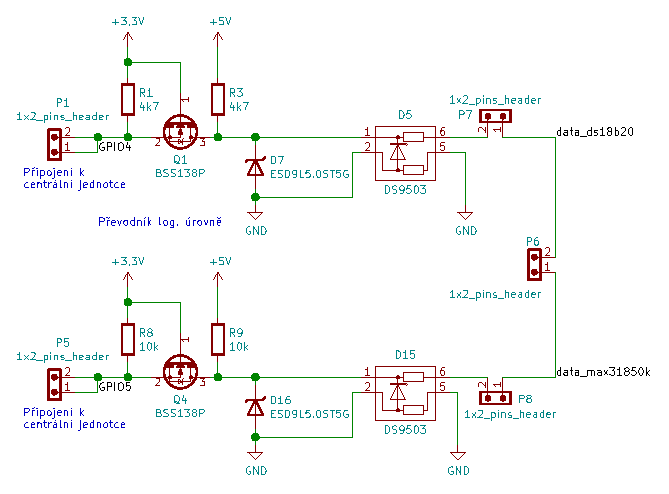
\includegraphics[width=\textwidth]{images/svg/kicad/ochrany-1-wire.eps}
    \caption[ESD ochrany pro 1-Wire sběrnici s~převodním napěťových úrovní]{ESD ochrany pro 1-Wire sběrnici s převodním napěťových úrovní. Kolíková lišta P1, P5 je připojena na Raspberry Pi.}
    \label{fig:ochrany-1-wire}
\end{figure}


\subsubsection{Napájení 1-Wire sběrnice}
\label{sec:napajeni-1-wire-sbernice}
Pro ochranu napájení 1-Wire sběrnice (5 V) jsou veškerá koncové teplotní senzory napájené přes elektronickou pojistku od Texas Instrumenst s označením TPS2600, obrázek \ref{fig:ochrana-napajeni-1-wire}. Která zajišťuje ochranu pro vstupní napětí, hlídá maximální hodnotu vstupního napětí do nastavené meze 5,25 V (maximální hranice je 60 V), minimální vstupní napětí do nastavené meze 4,75 V (minimální hranice je -60 V). Vstupní omezení napětí je pomocí rezistorů R5, R10, R11 a R12. Omezovací proud je nastaven na přibližně 73 mA (hodnotu lze změnit přes potenciometr R17), při jeho překročení dojde k odpojení výstupu pod dobu dokud nedojde k odstranění závady. Kondenzátor C2 nastavuje rychlost náběhu výstupního napětí. Pro indikaci chyb napájení je zde červená LED.

\begin{figure}[H]
    \centering
    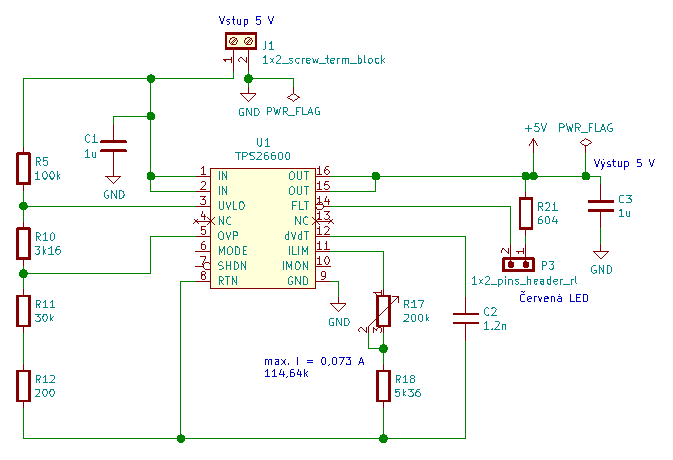
\includegraphics[width=\textwidth]{images/svg/kicad/ochrana-napajeni-1-wire.eps}
    \caption{Obvod TPS26600 pro ochranu napájení 1-Wire sběrnice.}
    \label{fig:ochrana-napajeni-1-wire}
\end{figure}

\subsubsection{Ochrana pro chodbové nástěnné termostaty}
Obdobně jako v části \ref{sec:datova-cast-1-wire-sbernice} (Datová část 1-Wire sběrnice) je stejná ochrana pro snímání logické úrovně z~chodbových nástěnných termostatů. Při sepnutí chodbového termostatu na daném patře je detekována log. 0 (požadavek na vytápění) v opačném případě je zde log. 1 (zastavení vytápění). Chodbové nástěnné termostaty jsou popsány v sekci \ref{digitalni-chodbove-termostaty}.

\subsubsection{Ochrana napájení 3,3 V}
Přímo z Raspberry Pi je využito napětí 3,3 V pro převodník napětí, popsaný v~části \ref{sec:datova-cast-1-wire-sbernice} (datová část 1-Wire sběrnice). Zde je použita vratná pojistka polymerový PTC (RXEF005) se spínacím proudem 100 mA, pro omezení proudu v~případě poruchy, dále je zde transilová dioda (SM2T3V3A) pro ochranu při přepětí (s~upínacím napětí max. 6,5 V (při 25 A, 10/1000~µs), průrazné napětí 3,6 V). Na obrázku \ref{fig:ochrana-napajeni-3_3-v} je zobrazena popsaná ochrana.

\begin{figure}[H]
    \centering
    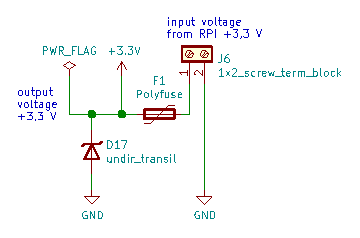
\includegraphics[width=0.6\textwidth]{images/svg/kicad/ochrana-napajeni-3_3-v.eps}
    \caption{Ochrana pro napájení 3,3 V z~Raspberry Pi.}
    \label{fig:ochrana-napajeni-3_3-v}
\end{figure}

\subsubsection{Způsob realizace 1-Wire sběrnice}
Samotná 1-Wire sběrnice je realizovaná pomocí UTP kabelu kategorie Cat5e. Na pinu číslo 4 jsou DATA, na pinu 5 je zem (GND) a na pinu 3 je napájení 5~V. Ze samotné DPS je sběrnice vyvedena pomocí konektorů RJ45, čtyři konektory pro teplotní senzory DS18B20 a čtyři pro termočlánky s MAX31850K.

\subsubsection{Realizovaná DPS ochran pro centrální jednotku Raspberry Pi}
Na obrázku \ref{fig:dps-rpi-1-wire-termostaty-ochrany-spodek} a \ref{fig:dps-rpi-1-wire-termostaty-ochrany-vrsek} je realizovaná DPS vstupů/výstupů pro centrální jednotku Raspberry Pi. Deska byla vlastnoručně navržena, vyrobena a osazena. Je aplikován ochranný lak, na vrchní propojky byl též aplikován ochranný lak a následně zakryty tavnou plastovou hmotou.

\begin{figure}[H]
    \centering
    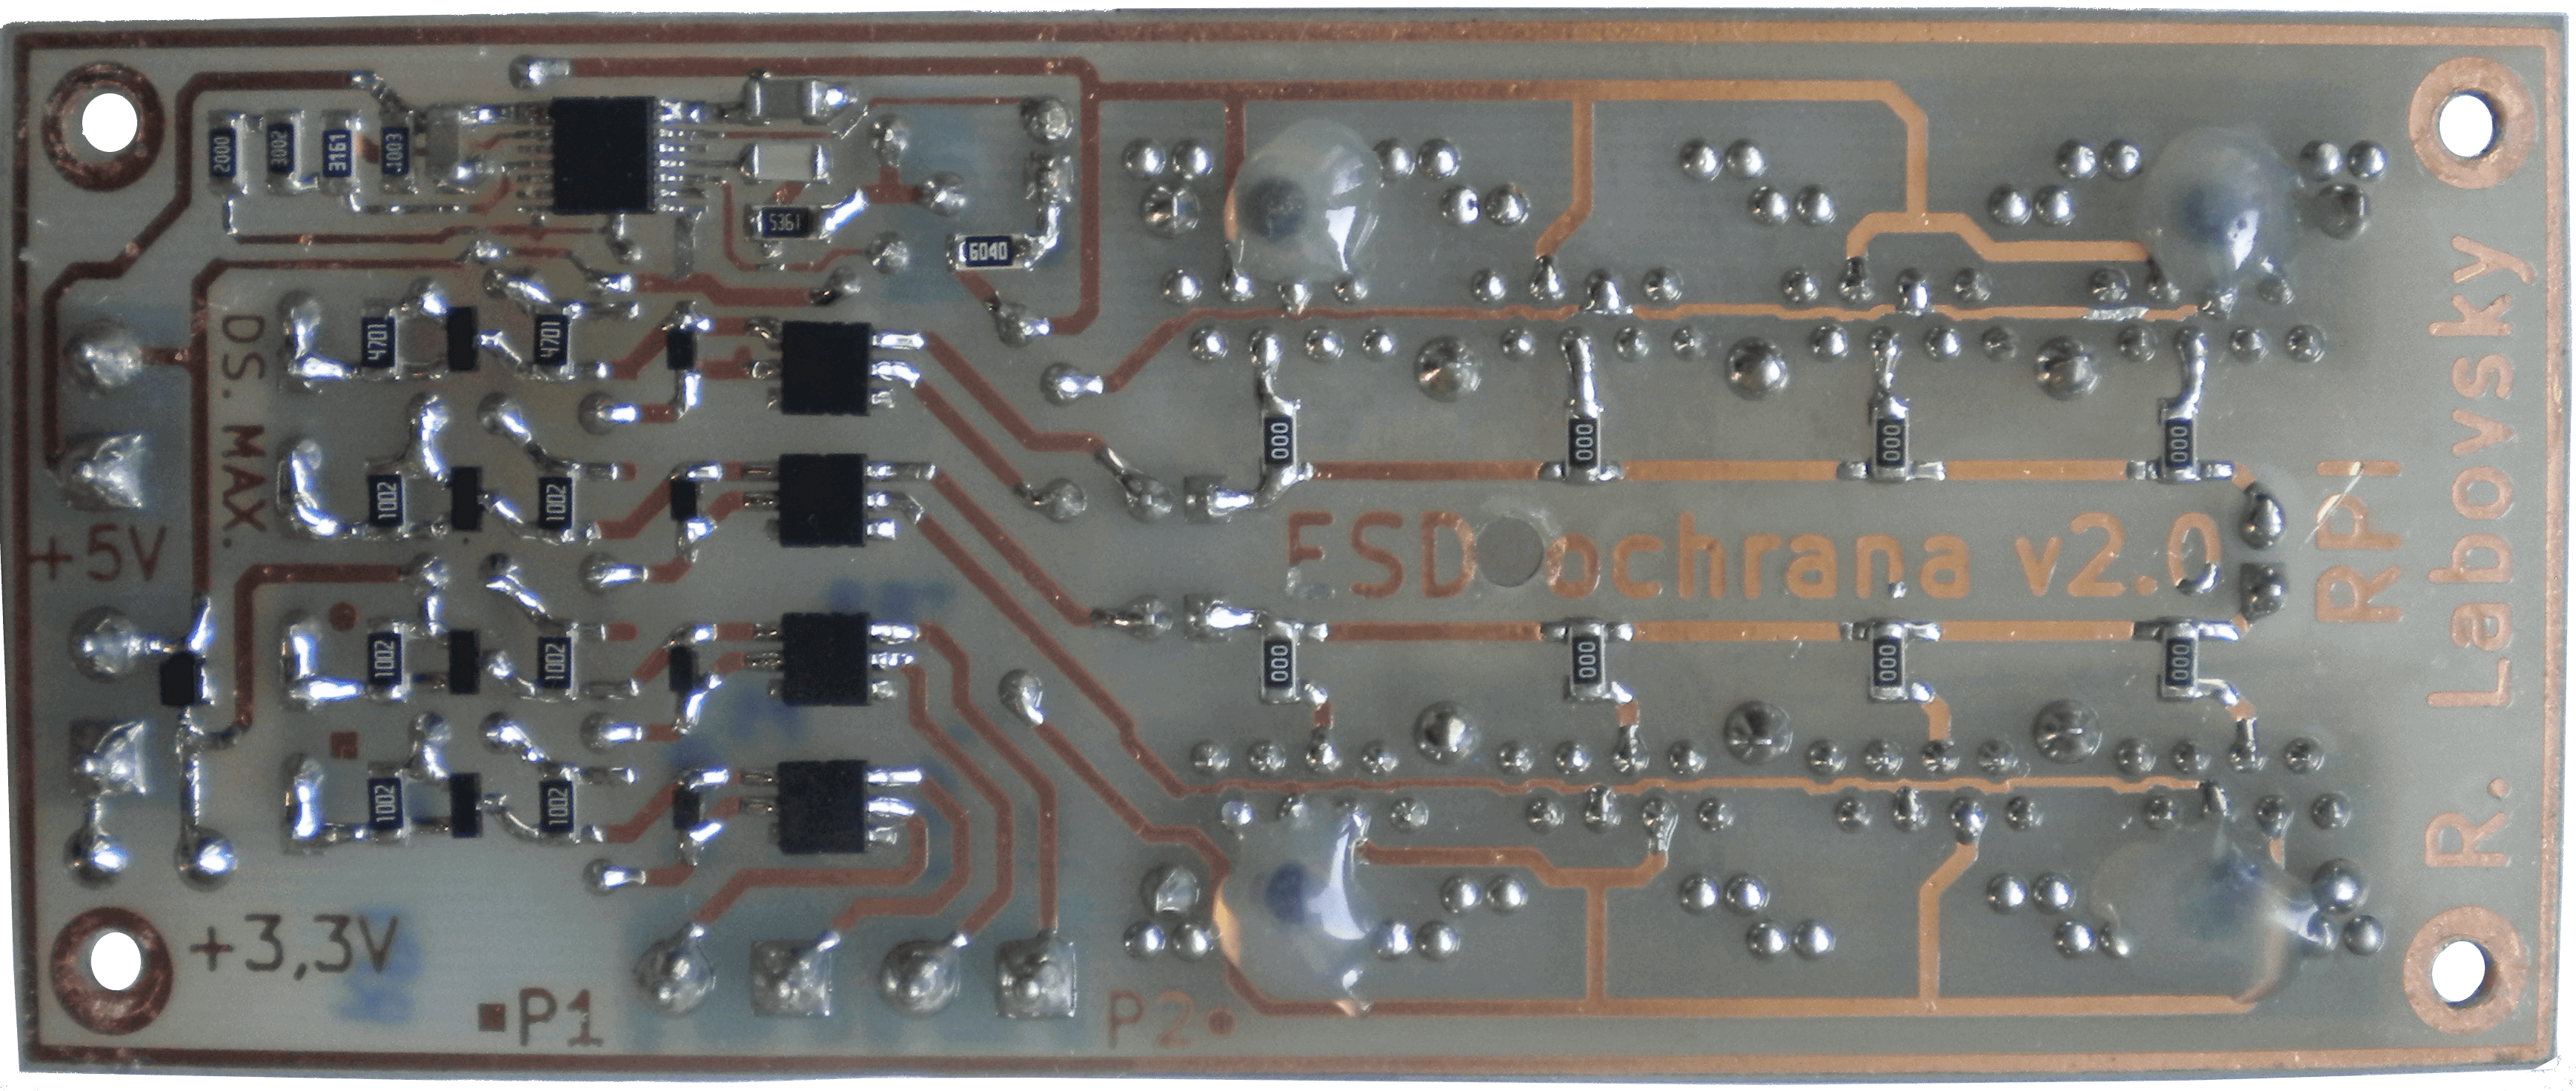
\includegraphics[width=\textwidth]{images/dps-rpi-1-wire-termostaty-ochrany-spodek.png}
    \caption{Spodní část DPS pro ochranu vstupů/výstupů pro centrální jednotku Raspberry Pi.}
    \label{fig:dps-rpi-1-wire-termostaty-ochrany-spodek}
\end{figure}

\begin{figure}[H]
    \centering
    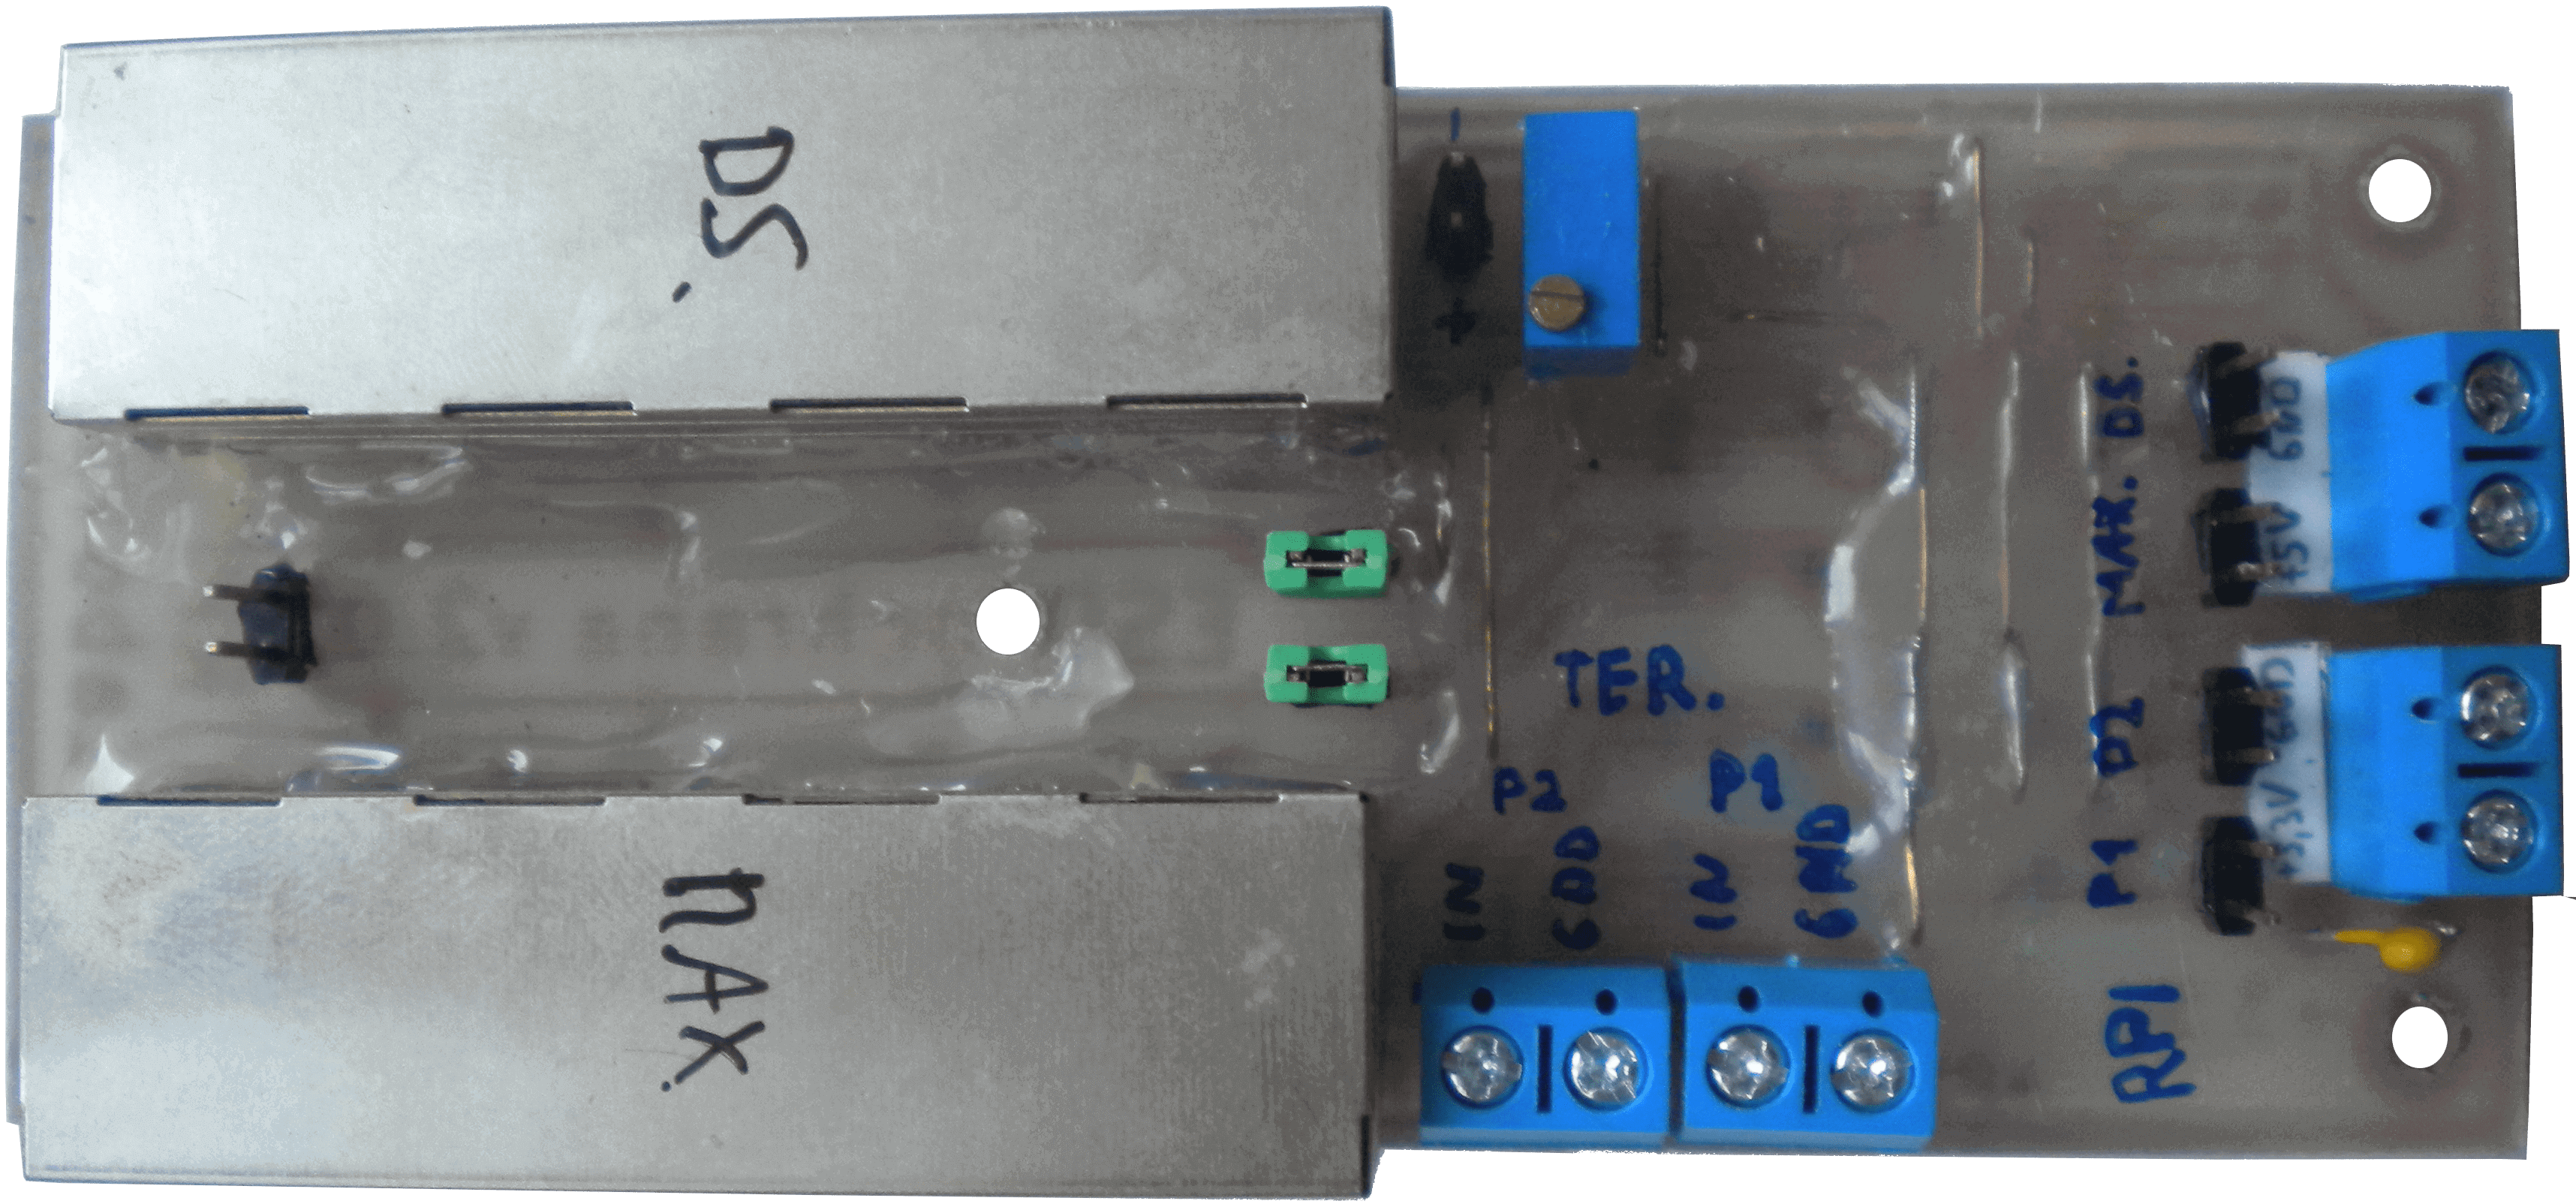
\includegraphics[width=\textwidth]{images/dps-rpi-1-wire-termostaty-ochrany-vrsek.png}
    \caption{Vrchní část DPS pro ochranu vstupů/výstupů pro Raspberry Pi.}
    \label{fig:dps-rpi-1-wire-termostaty-ochrany-vrsek}
\end{figure}

\section{DPS u krbů}
Navržená DPS se skládá z části elektronické pojistky TPS2600, zapojení je obdobné jako v \ref{sec:napajeni-1-wire-sbernice} (napájení 1-Wire sběrnice), navíc je na vstupu připojena transilová dioda (ESD9L5.0ST5G). Napěťové meze jsou nastaveny stejně, tedy minimální napětí je 4,75 V, maximální 5,25 V, proud je omezen na maximální hodnotu 100 mA. Dále je zde přivedena 1-Wire sběrnice přes konektor RJ45 s~obdobnými ochranami jako v \ref{sec:datova-cast-1-wire-sbernice} (datová část 1-Wire sběrnice), včetně stejných ochran pro napájení, pro připojení MAX31850K přes svorkovnici. V neposlední řadě jsou zde vstupy pro ovládání třech LED pro signalizaci (obrázek \ref{fig:ochrana-krby-lcd-teplotni-senzor}) naakumulovaného zásobníku otopné vody, modrá led signalizuje stav horní části zásobníku, oranžová LED je pro střední část, červená je pro signalizaci spodní části. Vstupní část je chráněná přes DS9503 a transilovou diodou (ESD9L5.0ST5G). Sepnutí LED je přes tranzistor (BSS138P). Obdobně jsou řešeny oranžová a modrá LED.

\begin{figure}[H]
    \centering
    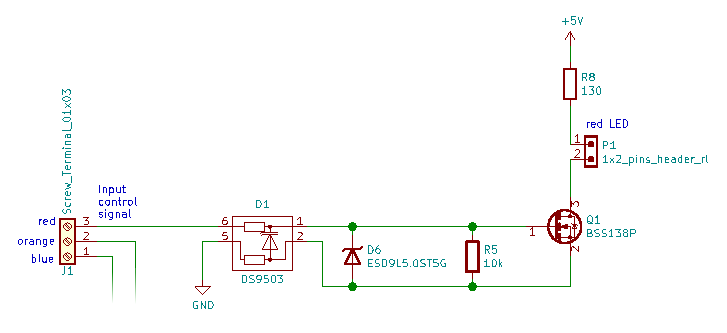
\includegraphics[width=\textwidth]{images/svg/kicad/ochrana-krby-lcd-teplotni-senzor.eps}
    \caption{Zapojení pro ovládání signalizační červené LED.}
    \label{fig:ochrana-krby-lcd-teplotni-senzor}
\end{figure}

\subsubsection{I$^2$C sběrnice}
\label{ses:i2c-sbernice}
Sběrnice I$^2$C je realizovaná pomocí zakoupeného modulu (obrázek \ref{fig:modul-pca9615-i2c-sbernice}) s~obvodem PCA9615 do firmy  NXP Semiconductors. Vstupní signál SCL a~SDA je veden přímo z~centrální jednotky na vstupu obovodu PCA9615, napájení je s 3,3 V logikou. Výstup z PCA9615 je pomocí diferenciální vedení, pro každý signál SCL a~SDA jsou použity dva vodiče. Napájení na této straně je pomocí 5 V. Sběrnice je realizovaná pomocí UTP Cat5e, výstup z~modulu je realizován pomocí konektoru RJ45. Vzhledem k použití UTP kabelu a diferenciálnímu přenosu je možné dosáhnout velké vzdálenosti sběrnice. Nejdelší bod dosahuje přibližně 30 m, je tedy možné použít I$^2$C sběrnici na vzdálenost pro kterou není standartě dělána. Použitá frekvence je 100~kHz. Jedná se tedy o plnohodnotnou I$^2$C sběrnici. Důvodem pro zvolení této varianty bylo na základě výběru displeje s I$^2$C sběrnicí (jednoduché a~levné řešení), dále jedná se o klasické zapojení displeje jako by se nalézal v~krátké vzdálenosti od centrální jednotky a není tak nutný převod jako při využít např. RS485 na UART a následně na I$^2$C sběrnici, v neposlední řadě komunikace je definována podle protokolu I$^2$C.  Jeden modul se nalézá na straně centrální jednotky a pak na straně krbů. Napájení 5 V je realizováno pomocí samostatných kabelů, není tedy součástí UTP kabelu. Z důvodu omezení kabeláže je sběrnice realizována v jednom UTP kabelu s 1-Wire sběrnicí, tedy přesněji jsou využity volné vodiče s číslem 1,2 pro SCL a 7,~8 pro SDA. Zařízení lze zapojovat jak na straně před PCA9615, tak i~na diferenciální straně, je však výhodné připojené uzly udržet co v nejkratší vzdálenosti kvůli degradování výkonu. Blokové schéma je na obrázku \ref{fig:blokove-schema-pca9615-i2c-sbernice} včetně napojení uzlů. Schéma zapojení modulu je na obrázku \ref{fig:zapojeni-pca9615-i2c-sbernice}.

\begin{figure}[H]
    \centering
    \def\svgwidth{\columnwidth}
    \input{images/svg/blokove-schema-pca9615-i2c-sbernice.pdf_tex}
    \caption[Blokové schéma zapojení obvodu PCA9615.]{Blokové schéma zapojení obvodu PCA9615 s impedančním zakončením sběrnice a možnostmi napojení uzlů. Upraveno z \cite{pca9615-schema-zapojeni}.}
    \label{fig:blokove-schema-pca9615-i2c-sbernice}
\end{figure}

\begin{figure}[H]
    \centering
    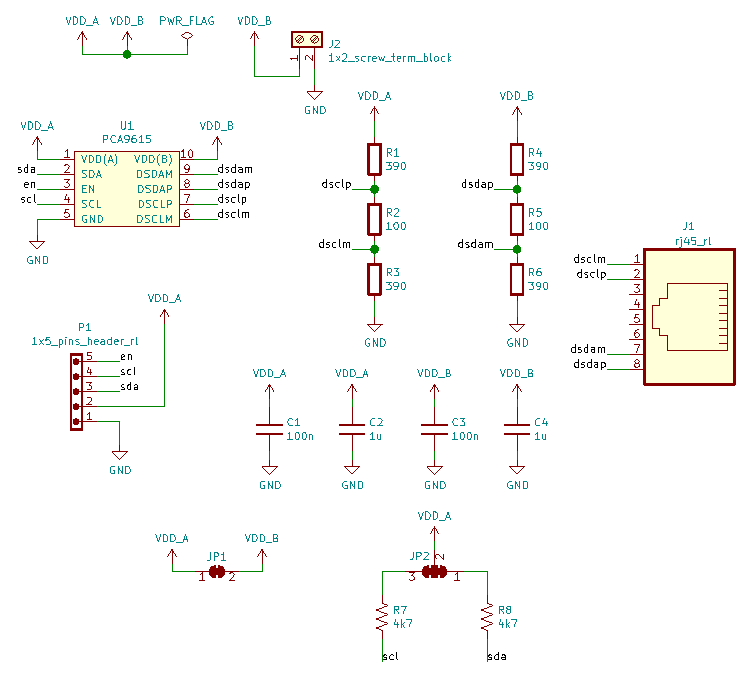
\includegraphics[width=\textwidth]{images/svg/kicad/zapojeni-pca9615-i2c-sbernice.eps}
    \caption[Zapojení PCA9615 v modulu.]{Zapojení PCA9615 v modulu. Upraveno z \cite{pca9615-schema-zapojeni}.}
    \label{fig:zapojeni-pca9615-i2c-sbernice}
\end{figure}

Výhodou PCA9615 je automatický výběr směru komunikace, není potřeba externího ovládání. Komunikace je možná až do rychlosti 1 MHz (přibližně pro 3 m), se zvýšenou délkou je však nutné rychlost snížit. Komunikace využívá standardního protokolu I$^2$C. ESD ochrana, v případě naindukování přepětí po cestě. Nezávislost napájení, je možné napájet koncová zařízení z jiného zdroje než Master. V neposlední řadě se jedná o jednoduché řešení bez nutných další zařízení na straně Slave, stačí pouze zapojit koncové zařízení s~podporou I$^2$C.

\begin{figure}[H]
    \centering
    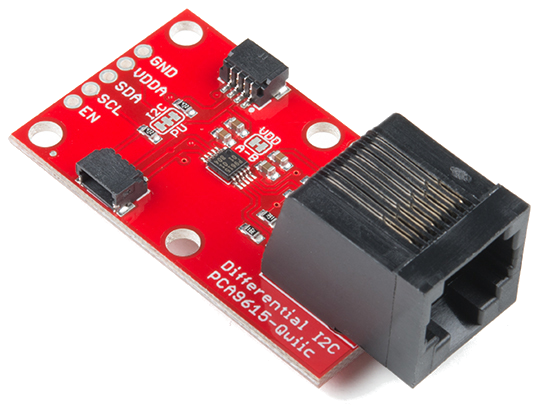
\includegraphics[width=0.6\textwidth]{images/modul-pca9615-i2c-sbernice.png}
    \caption[Modul s obvodem PCA9615.]{Modul s obvodem PCA9615 \cite{pca9615-i2c-modul}.}
    \label{fig:modul-pca9615-i2c-sbernice}
\end{figure}

\subsubsection{Měření teploty pomocí termočlánku a převodníku MAX31850K}
Teplotní senzory připojené na kouřovody krbů jsou realizované pomocí termočlánku z \ref{sec:teplotni-senzory-pro-krby}. Termočlánky jsou připojené k zakoupenému modulu (obrázek~\ref{fig:modul-max31850k-1-wire-prevodnik-termoclanku}) se zesilovačem napětí generované termočlánkem, hodnota napětí je následně převedena do digitální podoby včetně teplotní kompenzace studeného konce termočlánku a~tato hodnota je posílaná po 1-Wire sběrnici. Je možné připojit termočlánky typu K, J, N, S, R nebo E. Převodník umožňuje měřit teplotu s převodem pomocí AD převodníku až na 14 bitů. Rozlišení teploty činí 0,25 °C. Při teplotách -200 °C až 700 °C činí přesnost měřené teploty ±2~°C. Obvod disponuje detekcí zkratu (na GND nebo napájení) na vstupu pro termočlánek. Dále je zde detekci odpojeného termočlánku. Schéma zapojení modulu je na obrázku \ref{fig:zapojeni-max31850k-1-wire-prevodnik-termoclanku}.

\begin{figure}[H]
    \centering
    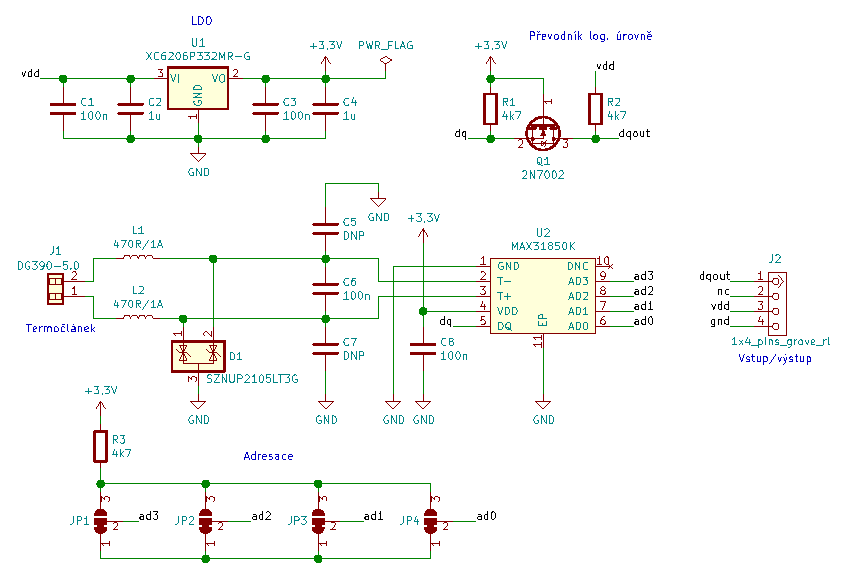
\includegraphics[width=\textwidth]{images/svg/kicad/zapojeni-max31850k-1-wire-prevodnik-termoclanku.eps}
    \caption[Zapojení MAX31850K v modulu.]{Zapojení MAX31850K v modulu. Upraveno z \cite{prevodnik-max31850k}.}
    \label{fig:zapojeni-max31850k-1-wire-prevodnik-termoclanku}
\end{figure}

\begin{figure}[H]
    \centering
    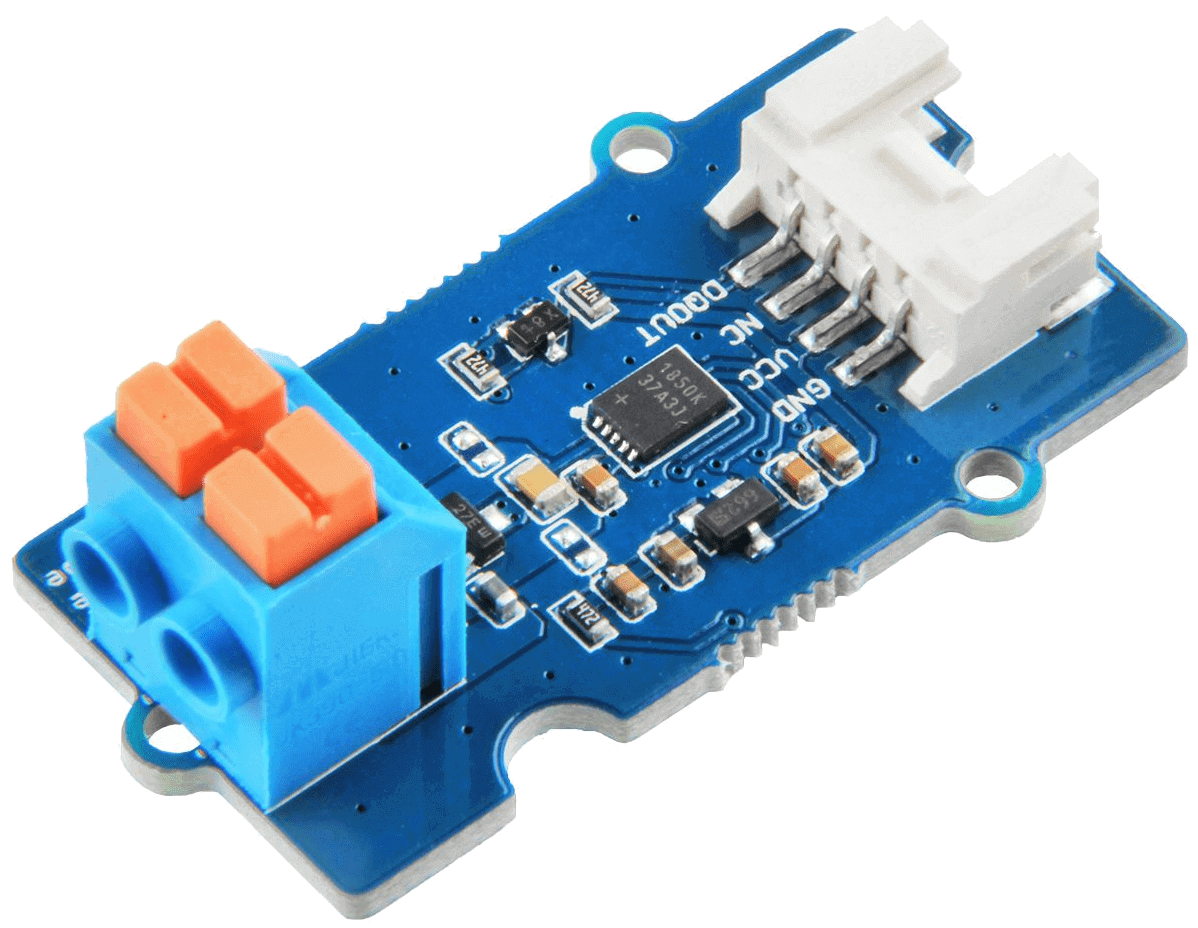
\includegraphics[width=0.6\textwidth]{images/modul-max31850k-1-wire-prevodnik-termoclanku.png}
    \caption[Modul s obvodem MAX31850K.]{Modul s obvodem MAX31850K \cite{prevodnik-max31850k}.}
    \label{fig:modul-max31850k-1-wire-prevodnik-termoclanku}
\end{figure}

\subsubsection{Realizace 1-Wire sběrnice u zásobníku otopné vody}
Na obrázku \ref{fig:dps-1-wire-sbernice-u-zasobniku-otopne-vody} je realizovaná DPS pro teplotní senzory u zásobníku otopné vody. Princip zapojení včetně ochrana na napájecí i datové části je popsán v~části \ref{sec:dps-se-vstupy-vystupy-pro-raspberry-pi} (datová část 1-Wire sběrnice). Na obrázku \ref{fig:instalacni-krabice-cidla-u-zasobniku-otopne-vody} je vidět horní část DPS vložená do instalační krabice. Celkově je zde k dispozici 6 pozic pro upevnění přes svorkovnice teplotní senzory. V současnosti jsou zde napojeny pouze 3 teplotní senzory (pro snímání teplot z horní, střední a spodní části zásobníku otopné vody). Na obrázku \ref{fig:ds18b20-ochrana} je teplotní senzor DS18B20 v~pouzdře TO-92 připevněn na UTP kabel a zataven plastovou hmotou na níž je následně nanesena smršťovací ochranná bužírka. Na obrázku \ref{fig:zasobnik-otopné-vody} jsou vyznačená místa s umístěním teplotních senzorů.

\begin{figure}[H]
    \centering
    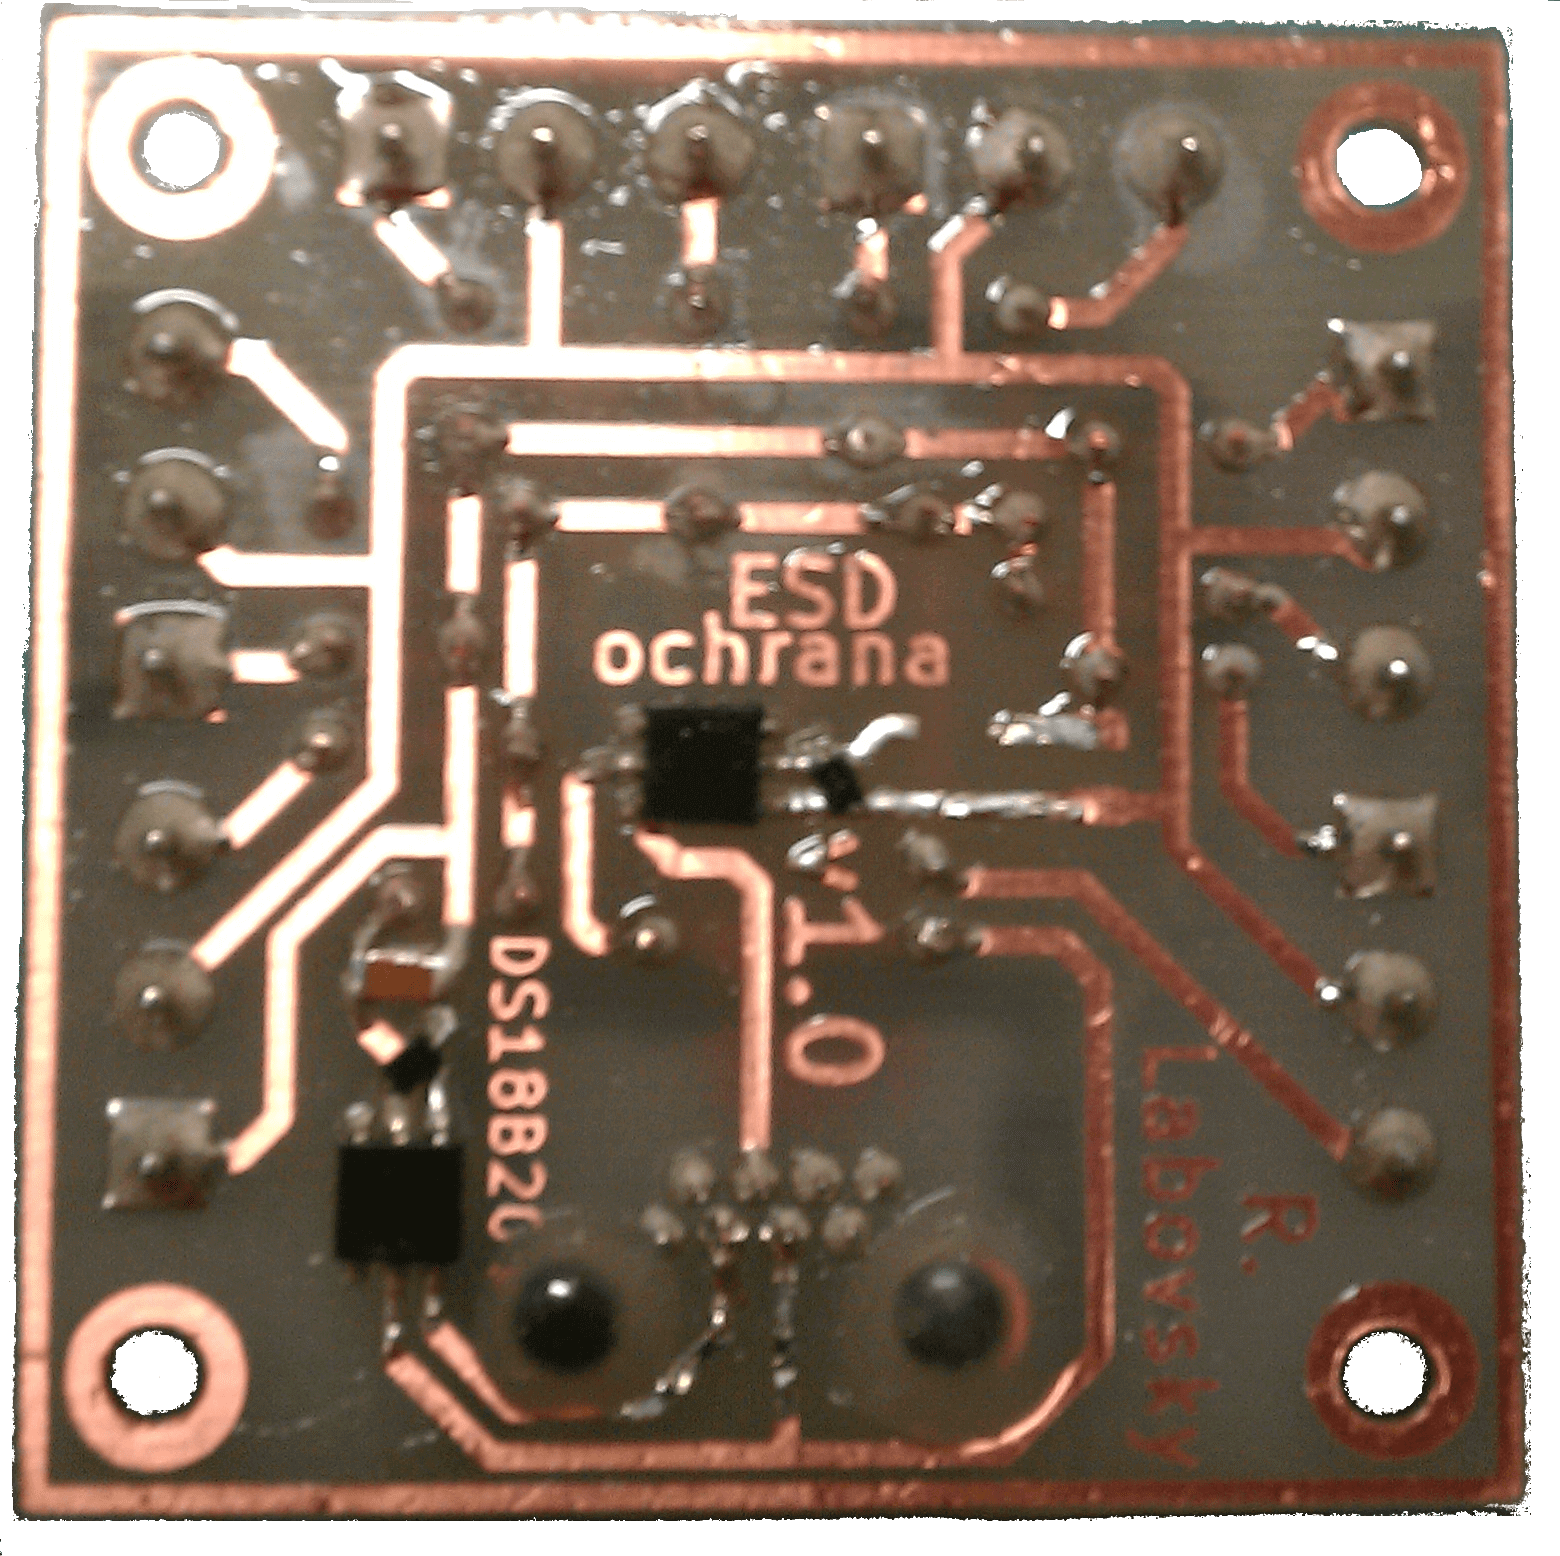
\includegraphics[width=0.6\textwidth]{images/dps-1-wire-sbernice-u-zasobniku-otopne-vody.png}
    \caption{Realizovaná DPS pro teplotní senzory 1-Wire sběrnice u zásobníku otopné vody.}
    \label{fig:dps-1-wire-sbernice-u-zasobniku-otopne-vody}
\end{figure}

\begin{figure}[H]
    \centering
    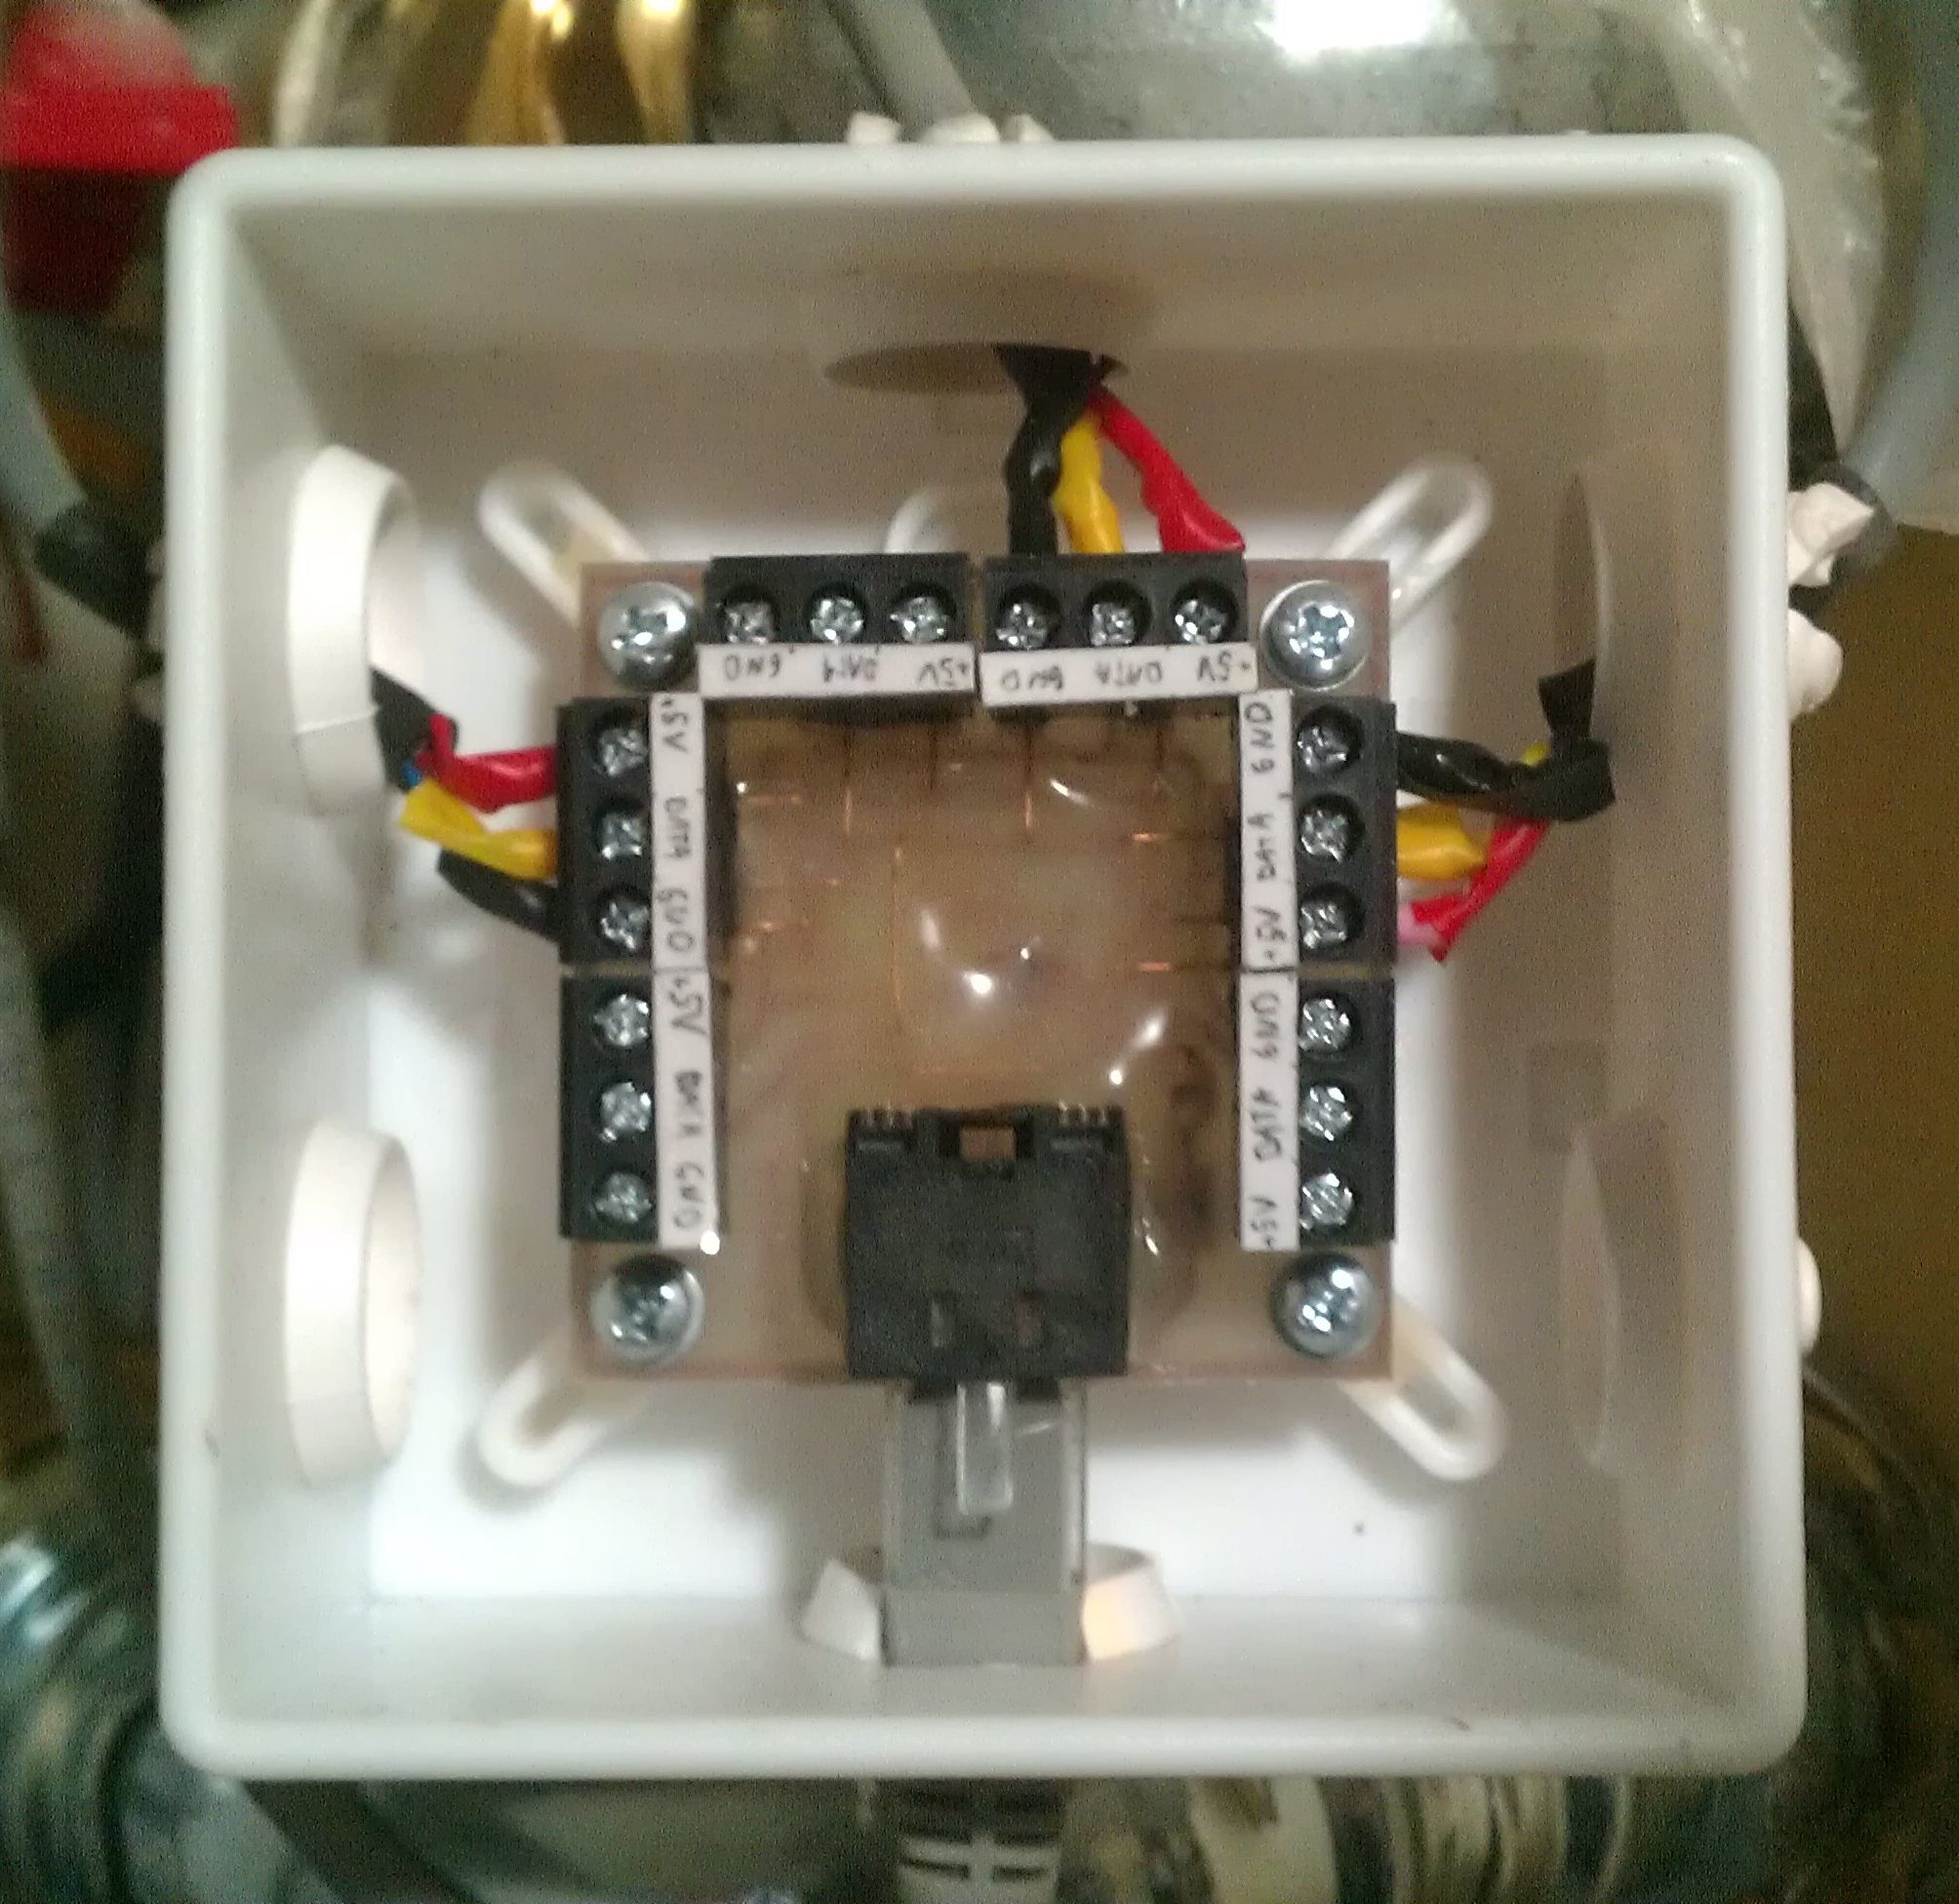
\includegraphics[width=0.6\textwidth]{images/instalacni-krabice-cidla-u-zasobniku-otopne-vody.png}
    \caption{Horní části DPS vložená do instalační krabice.}
    \label{fig:instalacni-krabice-cidla-u-zasobniku-otopne-vody}
\end{figure}

\begin{figure}[H]
    \centering
    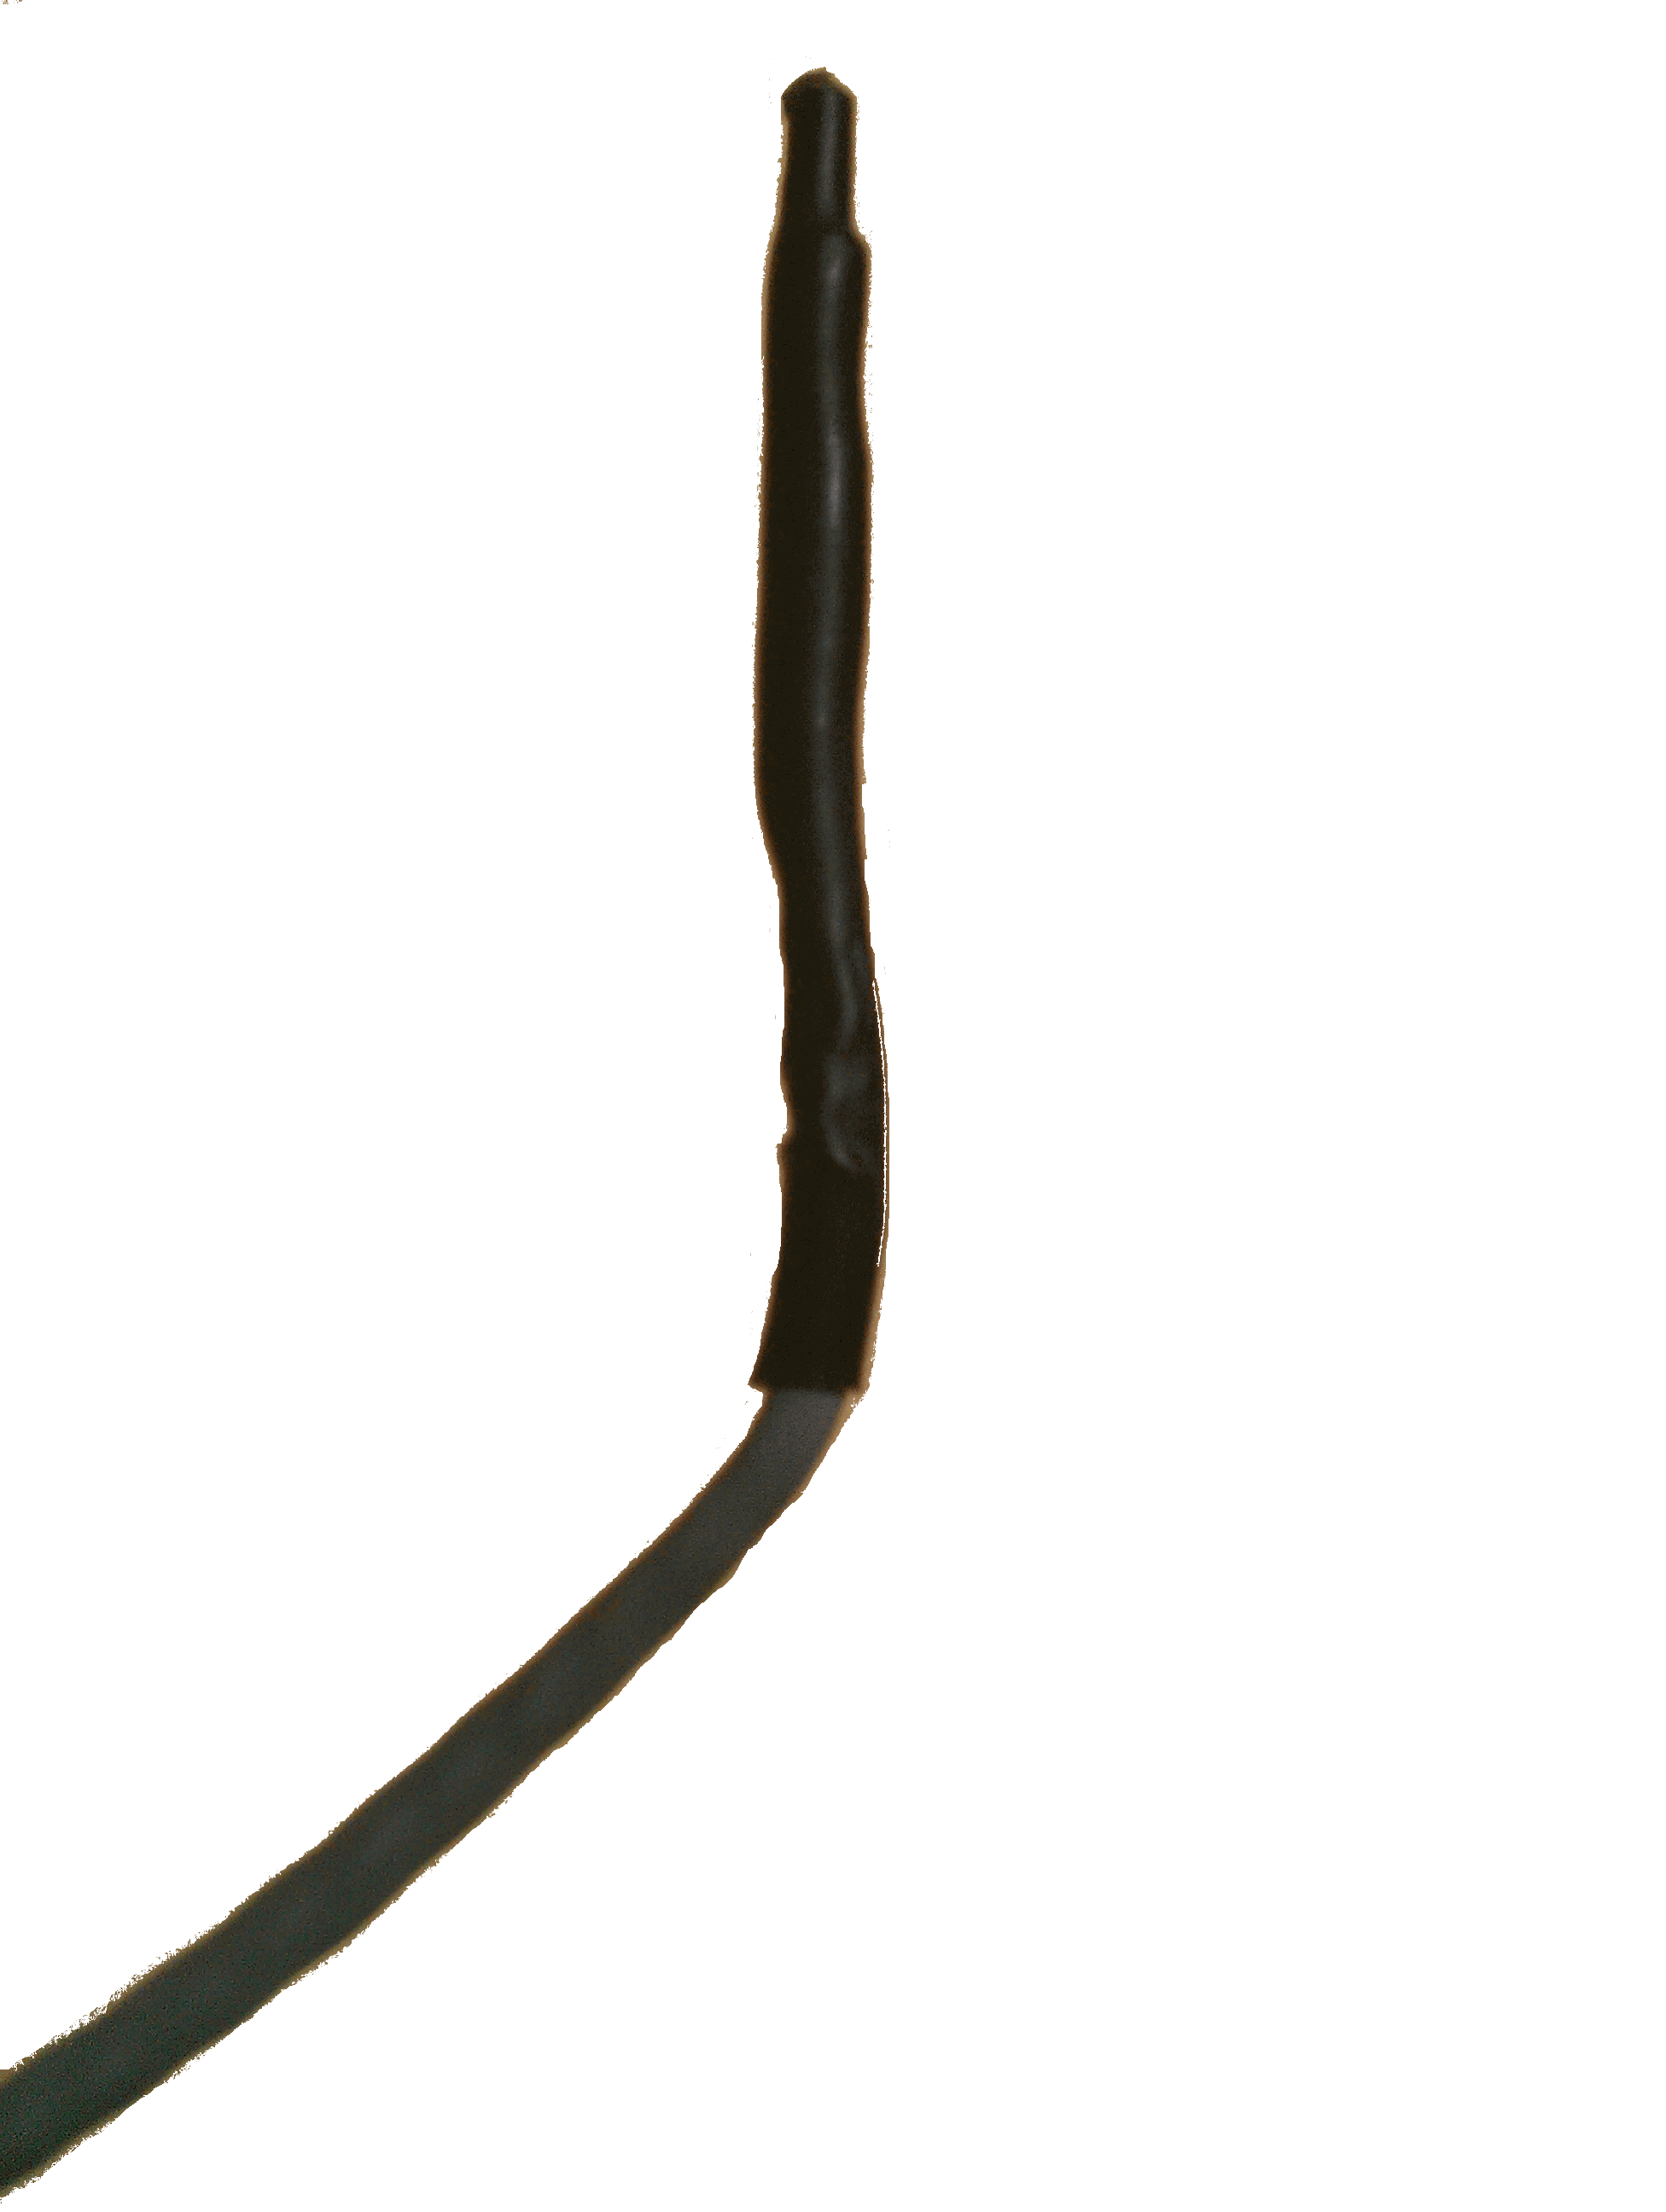
\includegraphics[width=0.6\textwidth]{images/ds18b20-ochrana.png}
    \caption{Teplotní senzor DS18B20 v~ochranném pouzdře.}
    \label{fig:ds18b20-ochrana}
\end{figure}

\begin{figure}[H]
    \centering
    \includegraphics[width=\textwidth]{images/zasobnik-otopné-vody.png}
    \caption[Zásobník otopné vody.]{Zásobník otopné vody. Červené kroužky označují místa teplotních senzorů.}
    \label{fig:zasobnik-otopné-vody}
\end{figure}


\subsubsection{LCD displej}
Pro zobrazování teplot ze střední a spodní části zásobníku otopné vody byl zvolen 16 znakový a 2 řádkový LCD displej s modrým podsvícením a~bílými písmeny (obrázek ). Po obsluhu displeje slouží řadič HD44780. K~řadiči je připojen I$^2$C expandér PCF8574 s osmi výstupy, které jsou připojená na datovou sběrnici pro ovládání respektive zobrazování znaků na displeji. Displej je zapojen za modulem popsaným v části \ref{ses:i2c-sbernice} (I$^2$C). Každý displej, respektive expandér PCF8574 umožňuje nastavit pomocí propojek A0, A1, A2 unikátní adresu zařízení na sběrnici.

\begin{figure}[H]
\centering
\begin{subfigure}{.5\textwidth}
  \centering
  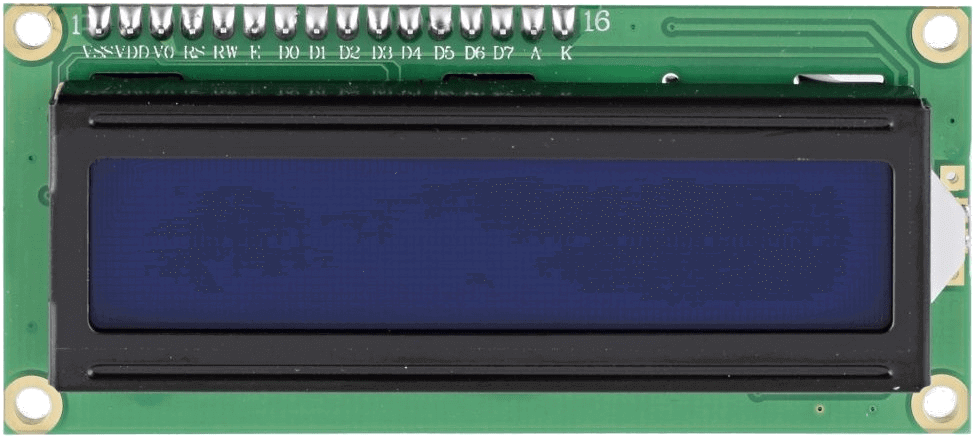
\includegraphics[width=0.9\linewidth]{images/predni-cast-lcd-displeje.png}
  \caption{Přední část displeje.}
  \label{fig:predni-cast-lcd-displeje}
\end{subfigure}%
\begin{subfigure}{.5\textwidth}
  \centering
  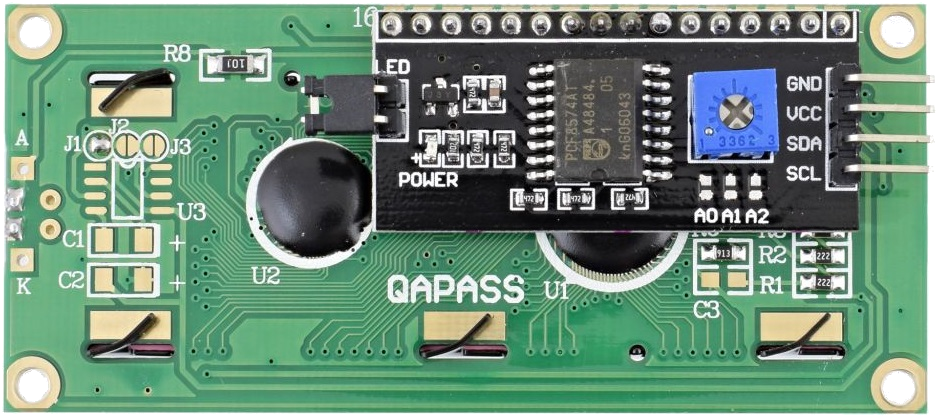
\includegraphics[width=0.9\linewidth]{images/zadni-cast-lcd-displeje-s-expanderem-pcf8574.png}
  \caption{Zadní část displeje s I$^2$C expandérem PCF8574.}
  \label{fig:zadni-cast-lcd-displeje-s-expanderem-pcf857}
\end{subfigure}
\caption[LCD displej pro zobrazování teplot ze zásobníku otopné vody.]{LCD displej pro zobrazování teplot ze zásobníku otopné vody \cite{lcd-displej}.}
\label{fig:lcd-displej}
\end{figure}

\subsubsection{Realizovaná DPS ochran a signalizace u krbů}

\begin{figure}[H]
    \centering
    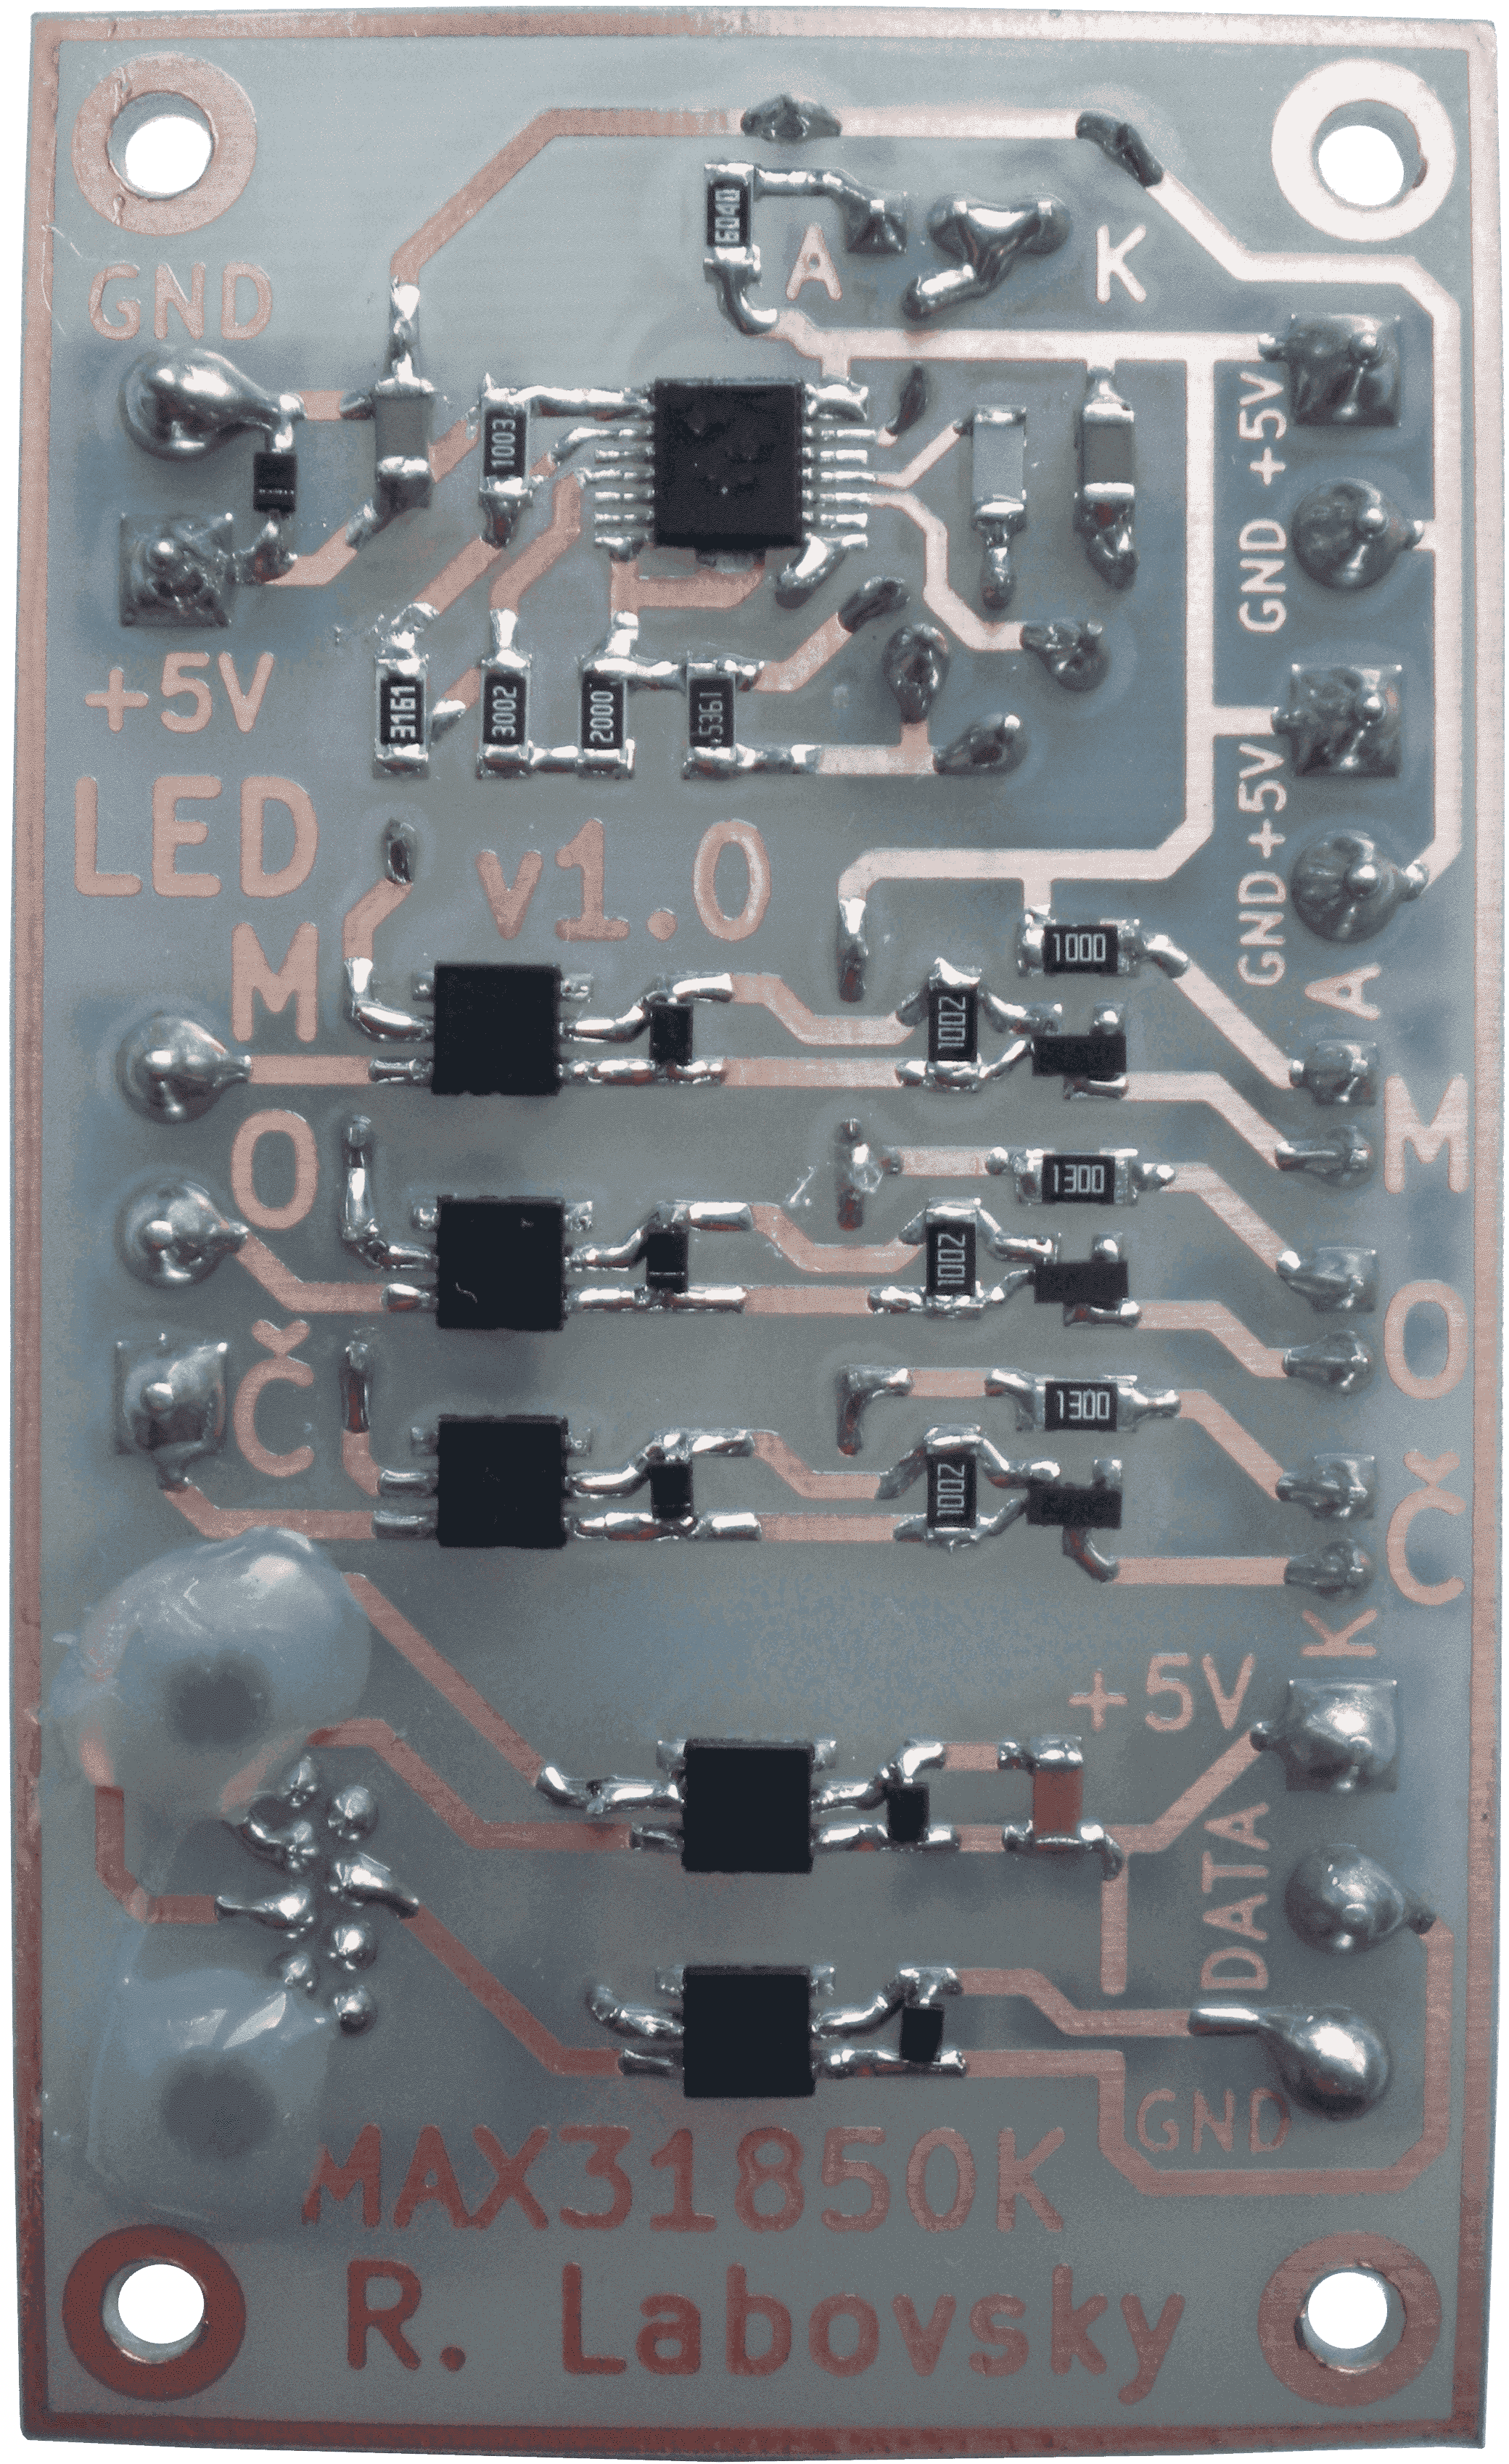
\includegraphics[width=\textwidth]{images/dps-led-ochrany-u-krbu-spodek.png}
    \caption{Spodní část DPS.}
    \label{fig:dps-led-ochrany-u-krbu-spodek}
\end{figure}

\begin{figure}[H]
    \centering
    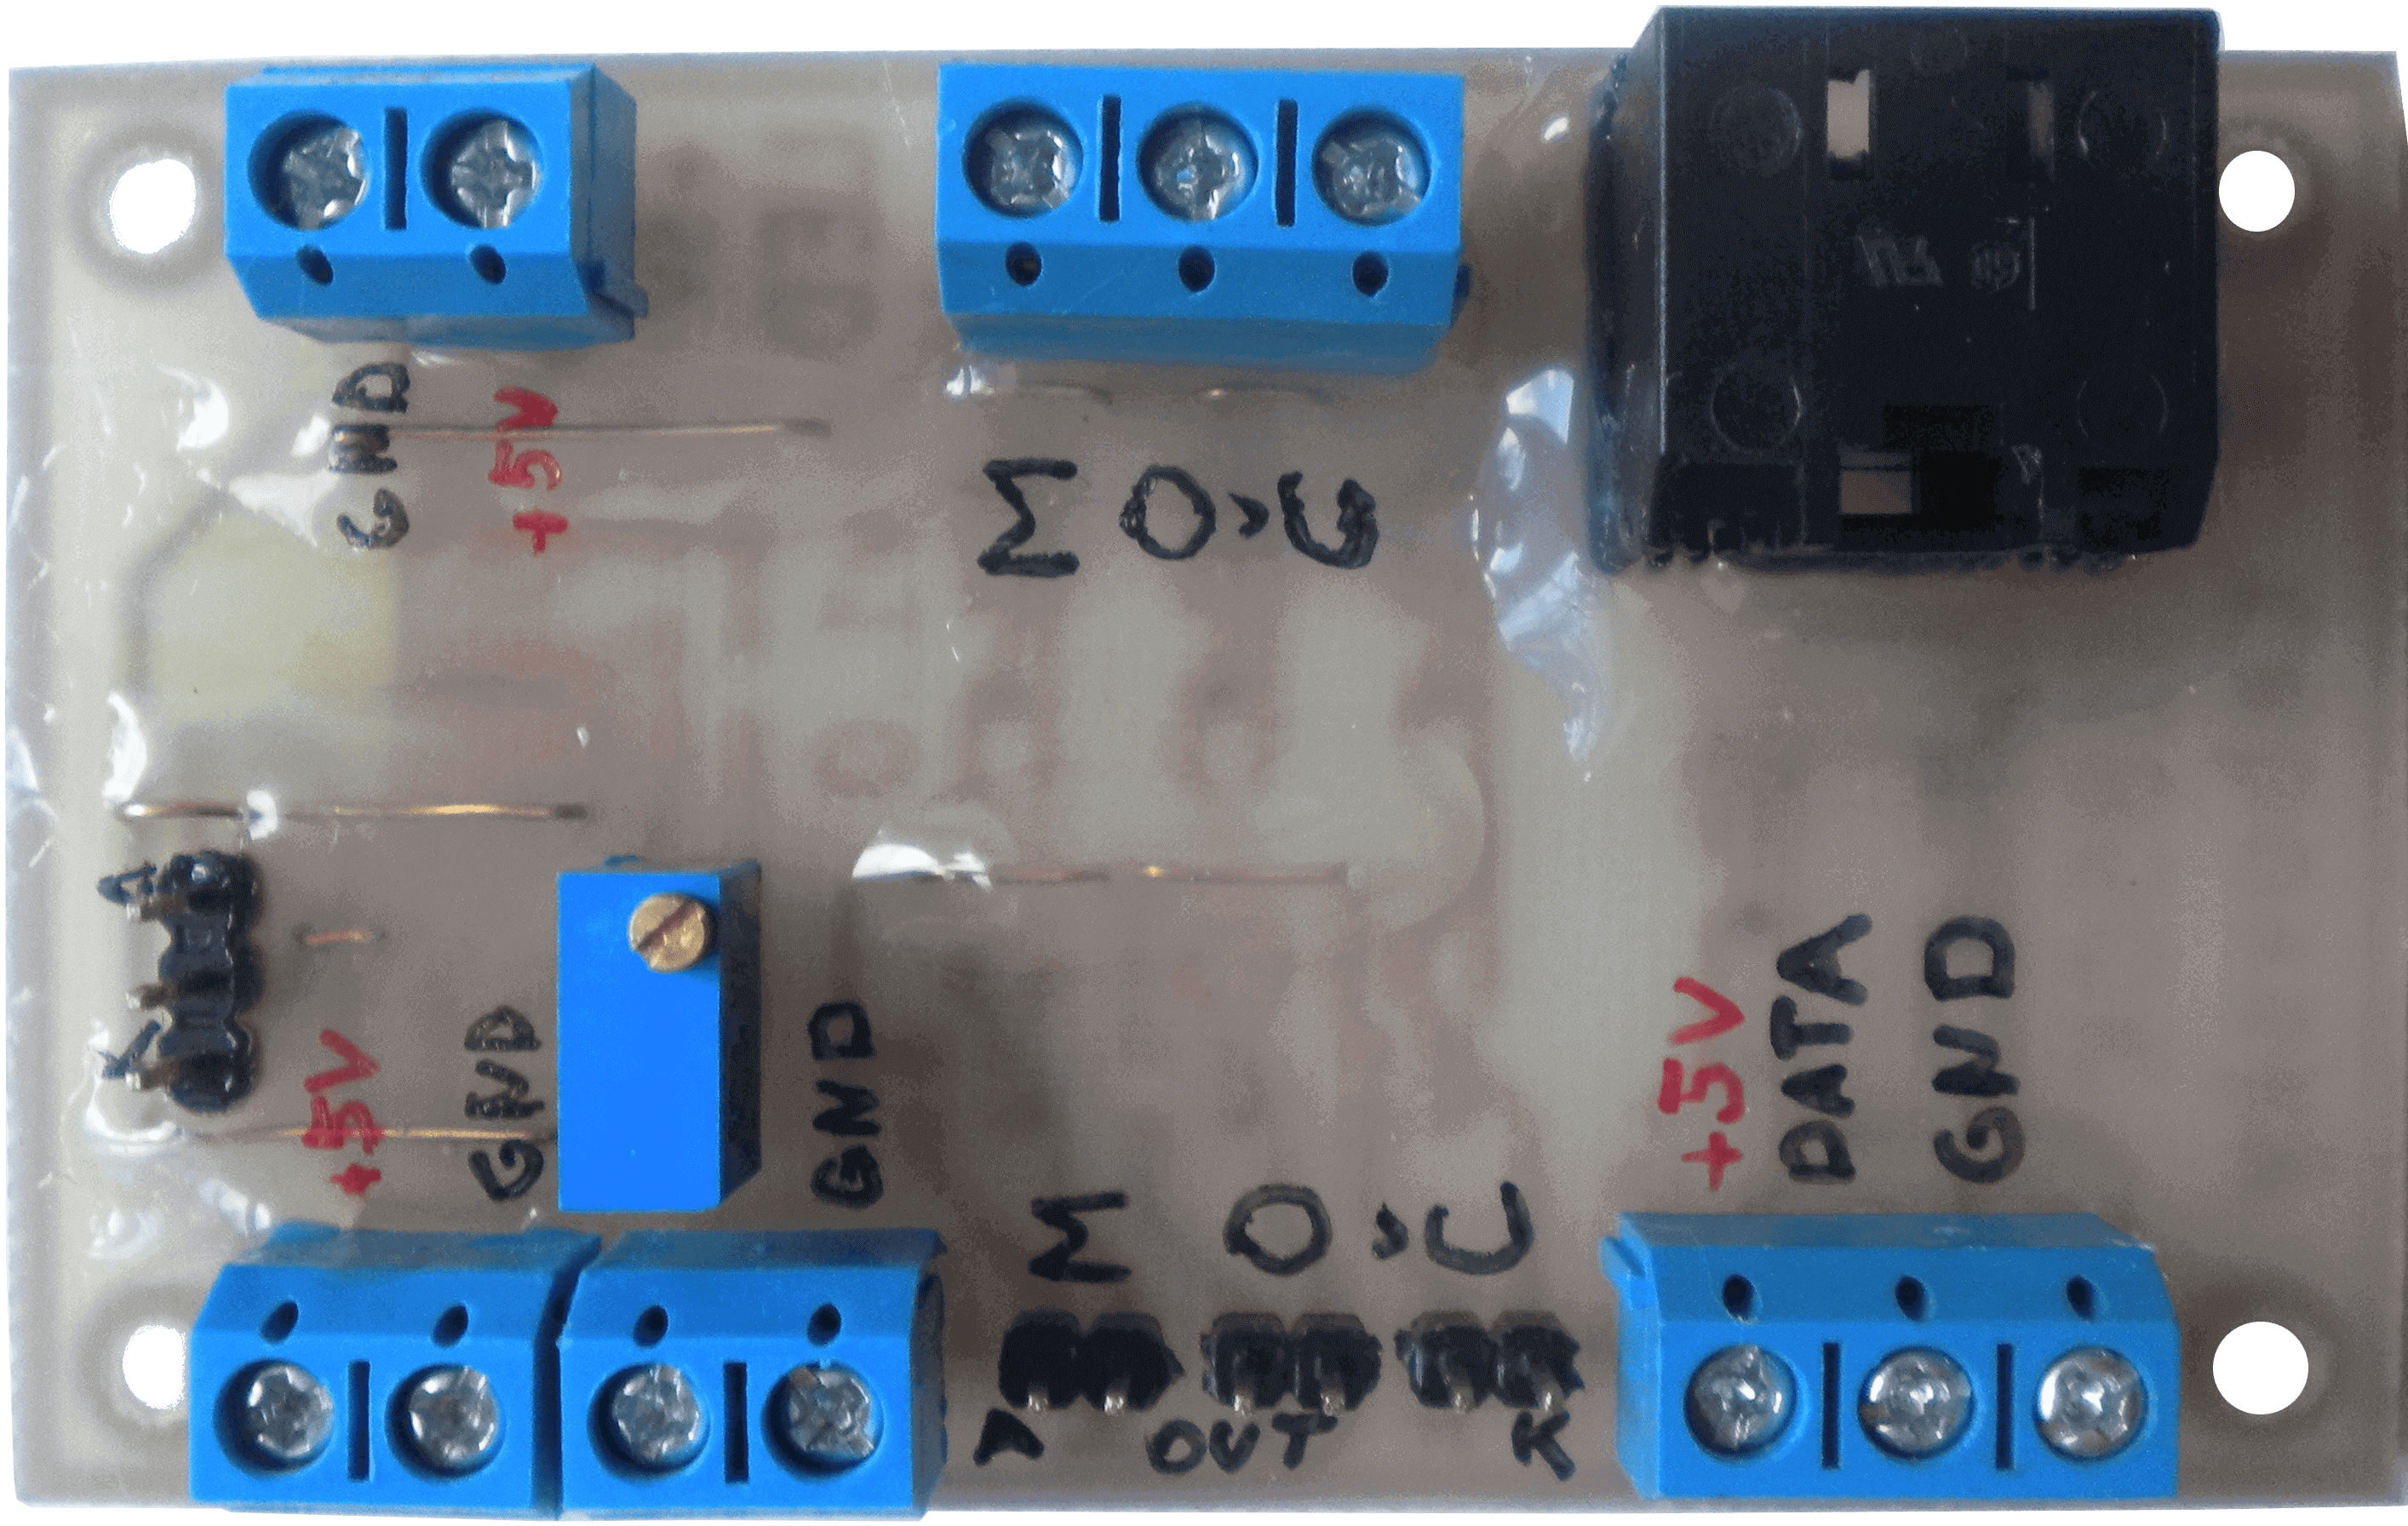
\includegraphics[width=\textwidth]{images/dps-led-ochrany-u-krbu-vrsek.png}
    \caption{Horní část DPS.}
    \label{fig:dps-led-ochrany-u-krbu-vrsek}
\end{figure}

\begin{figure}[H]
    \centering
    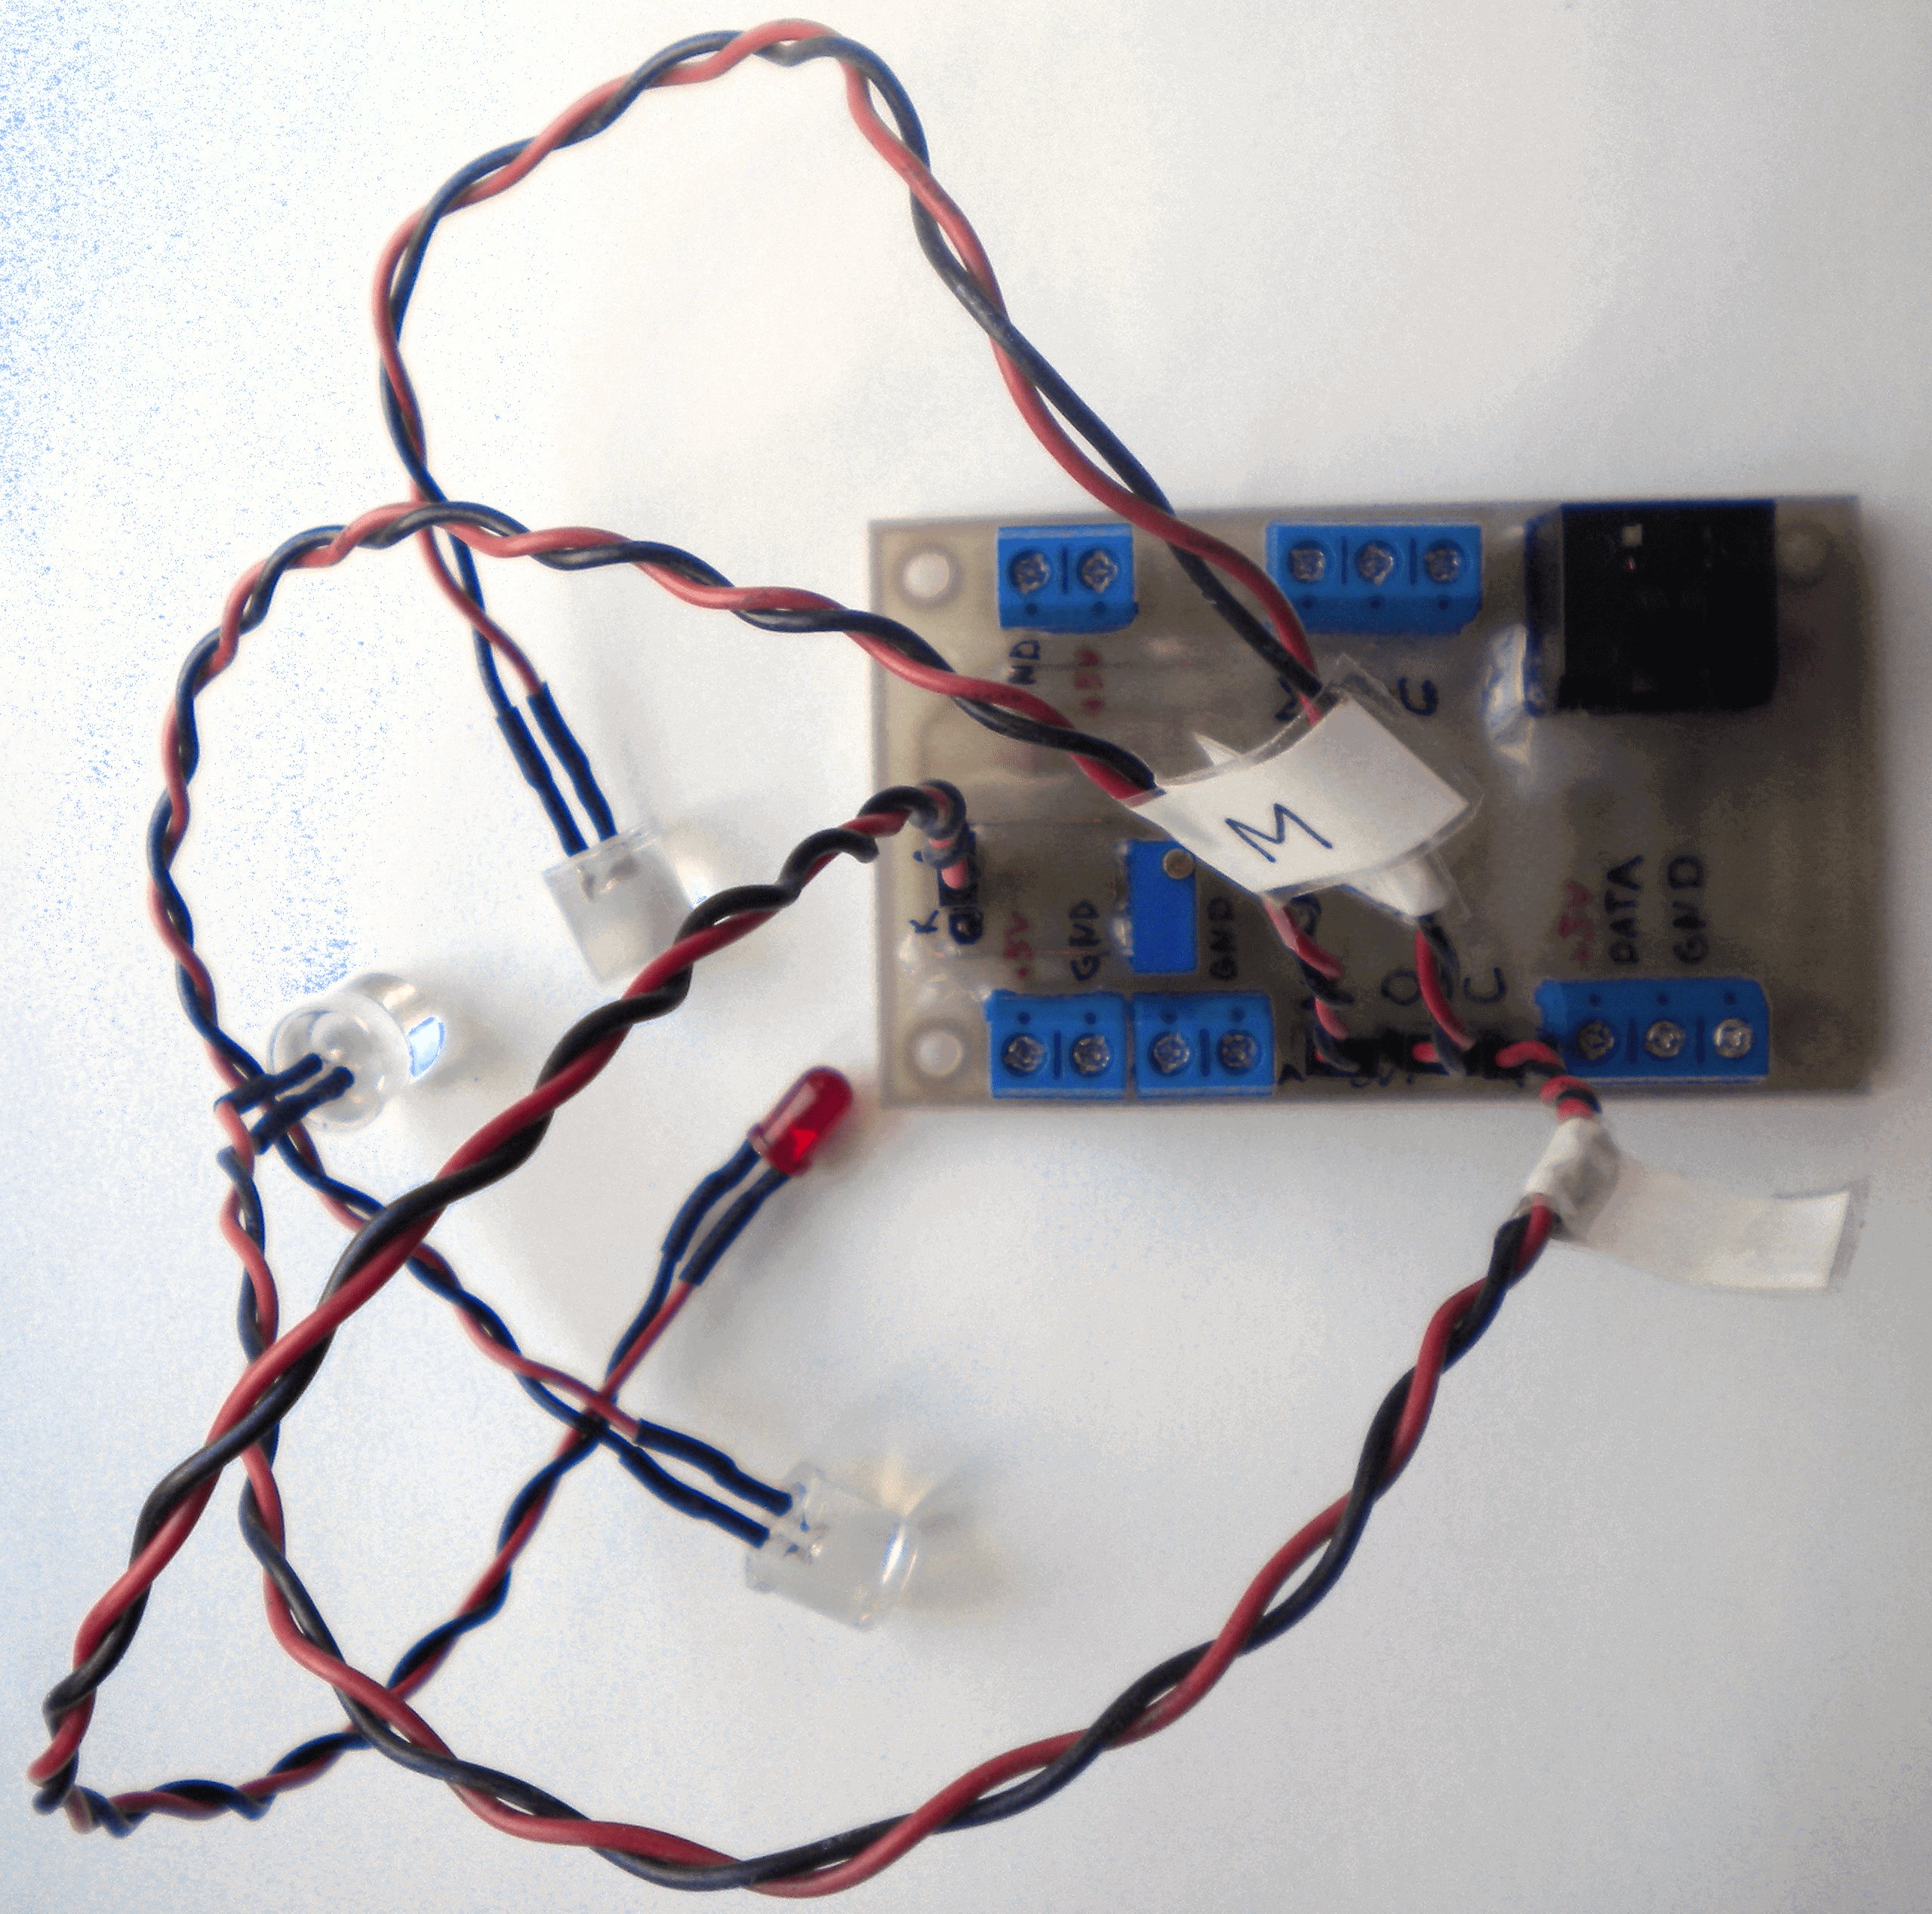
\includegraphics[width=0.95\textwidth]{images/dps-led-ochrany-u-krbu-kabely.png}
    \caption{DPS včetně signalizačních LED.}
    \label{fig:dps-led-ochrany-u-krbu-kabely}
\end{figure}

\subsubsection{Instalační krabice}
Všechna elektronika je umístěna do ochranné instalační krabice (obrázek \ref{fig:instalacni-krabice-vnitrek-krb}). Do krabice vstupují dva vodiče pro napětí 5 V a zem, tři kabely pro ovládání signalizačních LED, UTP kabel se sběrnicí 1-Wire pro teplotní senzor (termočlánek) a I$^2$C sběrnicí. Na obrázku \ref{fig:zadni-cast-krytu-vika-instalacni-krabice-krb} je zobrazena zadní část víka instalační krabice s uchycením signalizačních LED a LCD displeje. Na obrázku \ref{fig:predni-cast-krytu-vika-instalacni-krabice-krb} je přední část víka instalační krabice.

\begin{figure}[H]
    \centering
    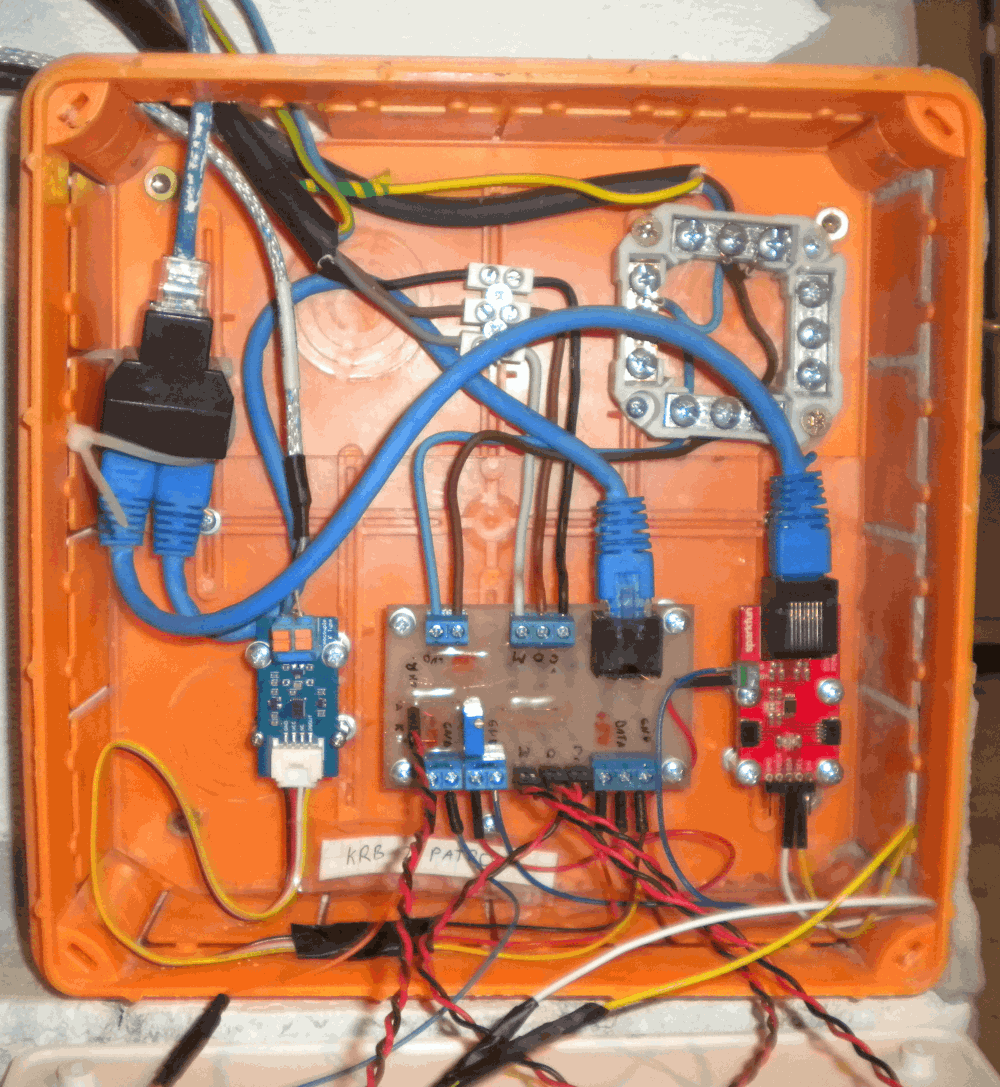
\includegraphics[width=0.6\textwidth]{images/instalacni-krabice-vnitrek-krb.png}
    \caption{Instalační krabice s jednotlivými moduly.}
    \label{fig:instalacni-krabice-vnitrek-krb}
\end{figure}

\begin{figure}[H]
    \centering
    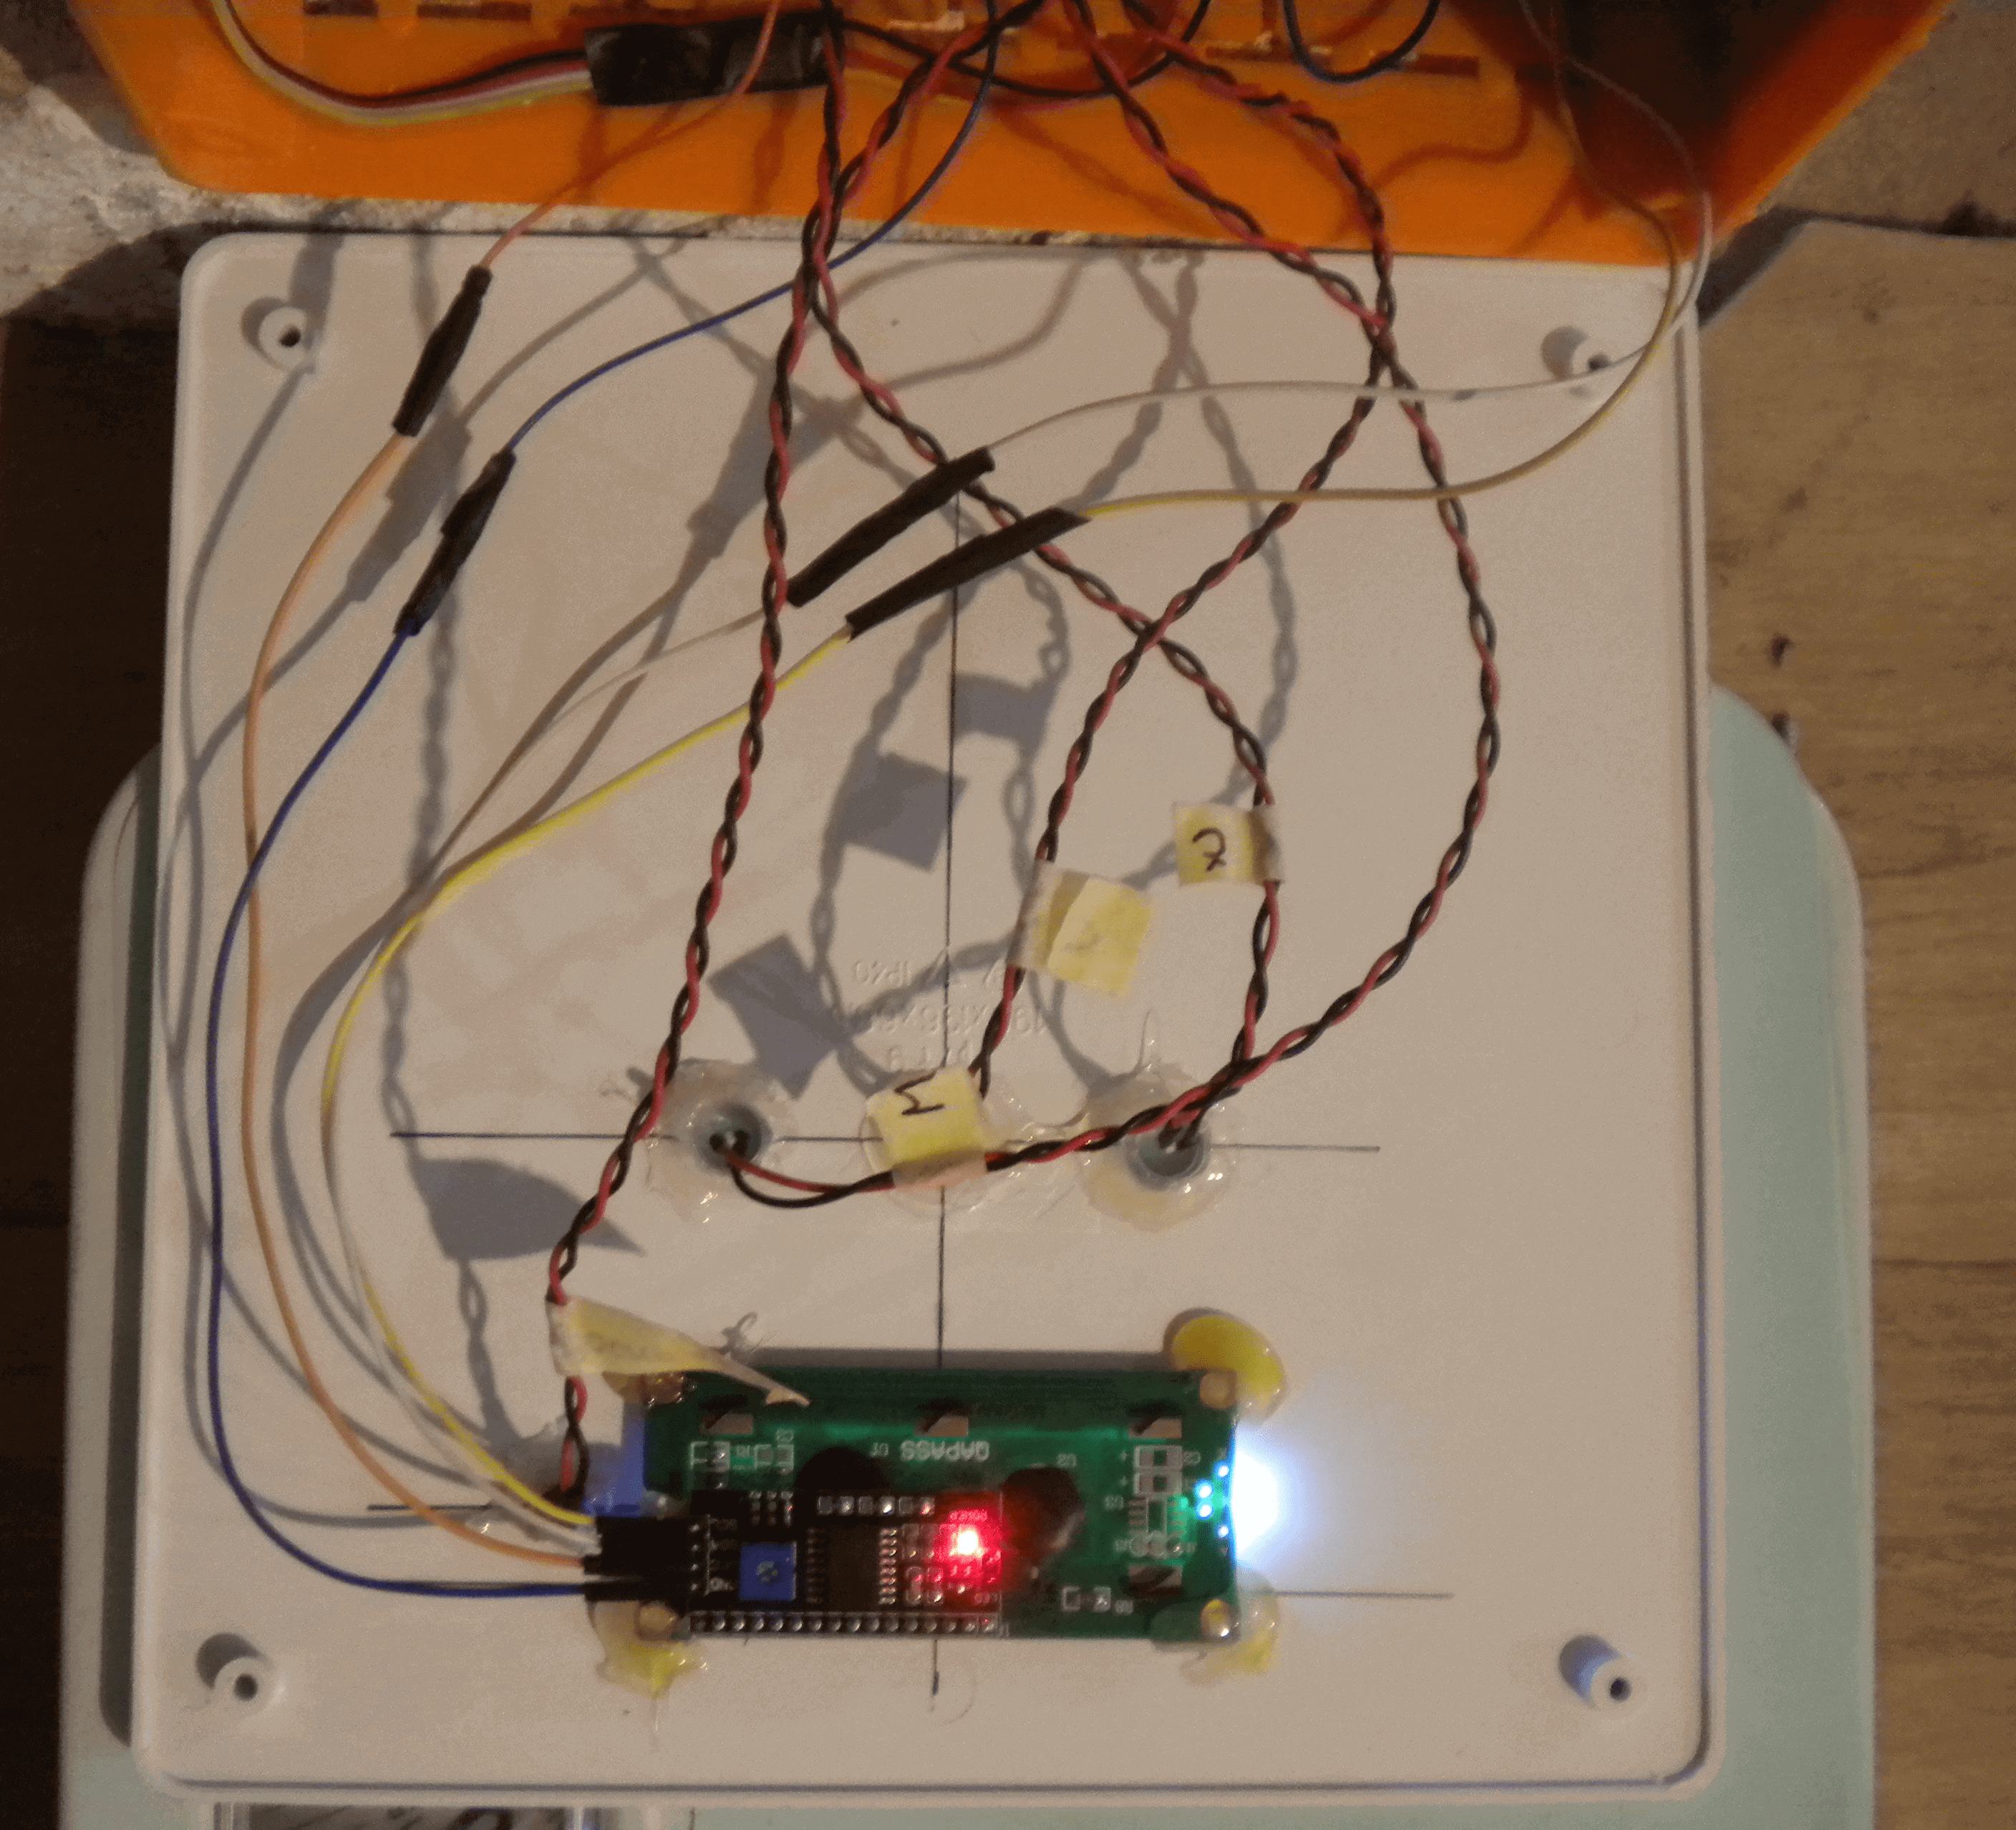
\includegraphics[width=0.6\textwidth]{images/zadni-cast-krytu-vika-instalacni-krabice-krb.png}
    \caption{Zadní část instalační krabice.}
    \label{fig:zadni-cast-krytu-vika-instalacni-krabice-krb}
\end{figure}

\begin{figure}[H]
    \centering
    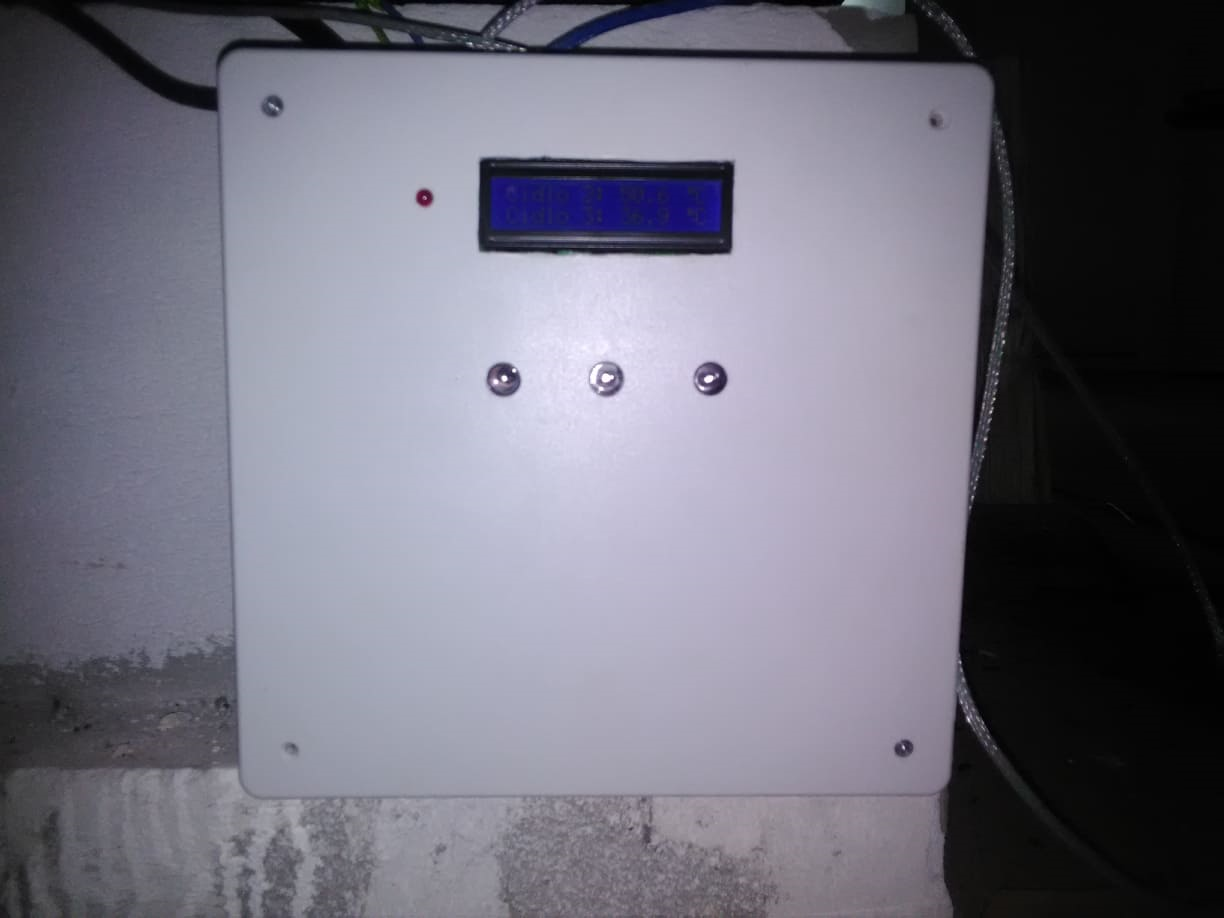
\includegraphics[width=0.6\textwidth]{images/predni-cast-krytu-vika-instalacni-krabice-krb.png}
    \caption[Víko instalační krabice.]{Víko instalační krabice. Osazený LCD displej, signalizačních LED (zleva modrá, oranžová a červená) a LED pro aktivování elektronické pojistky (červená LED vlevo od displeje).}
    \label{fig:predni-cast-krytu-vika-instalacni-krabice-krb}
\end{figure}

\section{Zónový regulátor}
Zónový regulátor se skládá s modulu PCA9615 (viz část \label{ses:i2c-sbernice} (I$^2$C)) pro realizaci I$^2$C sběrnice pomocí diferenciálních párů. Na modul je následně napojen zakoupený modul s obvodem PCA9685 od firmy NXP Semiconductors. Výstupy z modulu jsou napojeny na DPS, která zapíná/vypíná (respektive ke PWM regulaci) jednotlivé termoelektrické pohony (celkově 12 pohonů, každý je řízen samostatně), čímž dochází k regulaci otopné vody do otopných okruhů.

\subsubsection{Modul s PCA9685}
Modul s obvodem PCA9685 umožňuje pomocí I$^2$C sběrnice ovládat 16 výstupů se stejnou individuální hodnotou PWM (se střídou 0\% až 100 \%), frekvence je programovatelná od 24 Hz do 1\,526 Hz. Každý kanál navíc může dodat 10~mA jako source, případně 25 mA jako sink (což je 160 mA respektive 400~mA celkově).

\begin{figure}[H]
    \centering
    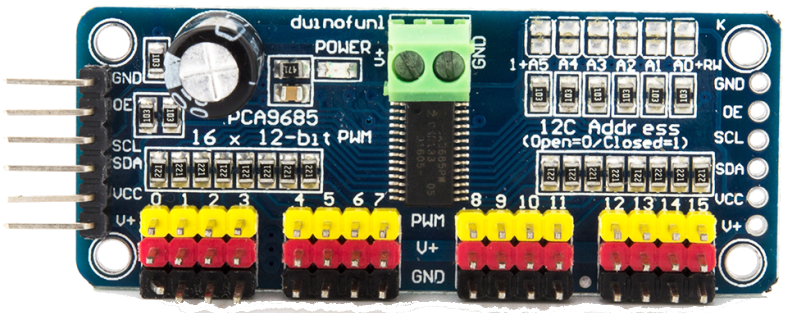
\includegraphics[width=0.8\textwidth]{images/modul-pca9685-pwm-regulace.png}
    \caption[Modul s obvodem PCA9685.]{Modul s obvodem PCA9685 \cite{modul-pca9685}.}
    \label{fig:modul-pca9685-pwm-regulace}
\end{figure}
\subsubsection{DPS pro ovládání termoelektrických pohonů}
Termoelektrické pohony jsou ovládány na základě hodnoty PWM z modulu PCA9685 (viz předchozí bod), každý výstupu ovládá jednotlivý pohon. Vzhledem k tomu, že termoelektrické pohony jsou na stejnosměrné napětí 24 V, je nutné využít napěťový převodník z 5 V na 24 V. K tomu slouží tranzistor MOSFET (DMN3023L-7). V závislosti na hodnotě PWM na jeho vstupu (gate) je otevírán/zavírán a dochází tak k regulaci napětí/proudu v~termoelektrickém pohonu, který je zapojen jako zátěž (přes drain). Paralelně k~tranzistoru se nachází přepínač, který slouží v případě poruchy k manuálnímu zapnutí/vypnutí pohonu. Přepínač má jmenovitý proud 0,5~A, což je dostatečné pro termoelektrický pohon, kterým při zapnutí teče maximální proud 250 mA (následně dochází ke snižování a saturaci proudu). Každý kanál obsahuje zelenou LED pro signalizaci, zda dochází k ovládání pomocí PWM. Maximální proud procházející zelenou LED je 7 mA, což je v~mezích pro obvod PCA9685, kde je uváděno, že pro každý kanál je maximální proud 10 mA. Jak již bylo řečeno pohony jsou napájeny pomocí 24 V, jsou vytvořené dvě napájecí větve s obvodem TPC26600 (popsaný v části \ref{sec:napajeni-1-wire-sbernice}), rozdíl spočívá ve vstupním napájení, které činí 24 V. Jsou tedy rozdílné i~maximální a~minimální povolené meze, které činí max. 24,25 V a min. 23,75~V. Dále každá větev má nastavený maximální proud 1,5 A (každý pohon má maximální hodnotu proudu při zapnutí 250 mA pro celkově 6 pohonů na větev). Vzhledem k jednoduchosti obvodu TPS26600 a k jeho vlastnostem (především pro automatickou detekci odstranění závady, bez nutnosti restartu zařízení) bylo raději zvoleno zapojení se dvěma větvemi (maximální proud pro TPS26600 činí 2,21 A) než využití jiného integrovaného obvodu pro sloučení do jedné větve. Na obrázku \ref{fig:dps-zonovy-regulator} je navržená DPS zónového regulátoru, která v současné době není vyrobená.


\begin{figure}[H]
    \centering
    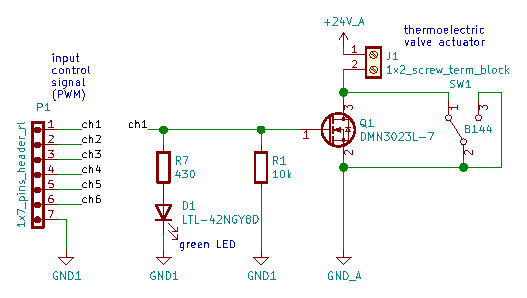
\includegraphics[width=\textwidth]{images/svg/kicad/zonovy-regulator-mosfet-pwm.eps}
    \caption{Zapojení jednoho kanálu pro ovládání termoelektrického pohonu.}
    \label{fig:zonovy-regulator-mosfet-pwm}
\end{figure}


\begin{figure}[H]
    \centering
    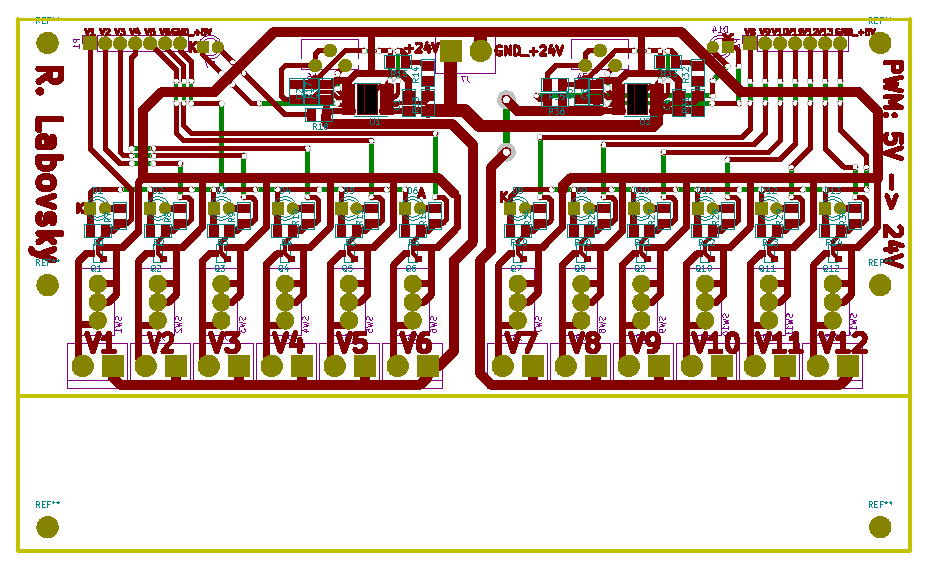
\includegraphics[width=\textwidth]{images/svg/kicad/dps-zonovy-regulator.eps}
    \caption[Navržená DPS pro zónový regulátor.]{Navržená DPS pro zónový regulátor. Rozměry jsou 151~mm~×~90~mm.}
    \label{fig:dps-zonovy-regulator}
\end{figure}

\subsubsection{Termoelektrické pohony Salus T30NC}  
Termoelektrický pohon Salus T30NC slouží k ovládání ventilů pro jednotlivé otopné okruhy. Je napájen stejnosměrným napětí 24 V při maximálním proudovém odběru při zapnutí 250 mA. Provozní příkon jsou 2 W. Rozměr závitu je M30\,×\,1,5. Maximální délka zdvihu pro dřík ventilu činí 4 mm. Síla pohonu je 100 N ($\pm$10 \%). Čas pro otevření je přibližně 2 minuty. Jedná se o~typ \acrshort{nc} (\textit{\acrlong{nc}}), při odpojení napájení je ventily zavřen. Pohon má funkci „First Open“ neboli je možné pomocí zarážky ventil instalovat jako otevřený bez nutnosti napájení (využít v případě, kdy není ještě instalovaná centrální jednotka).

\begin{figure}[H]
    \centering
    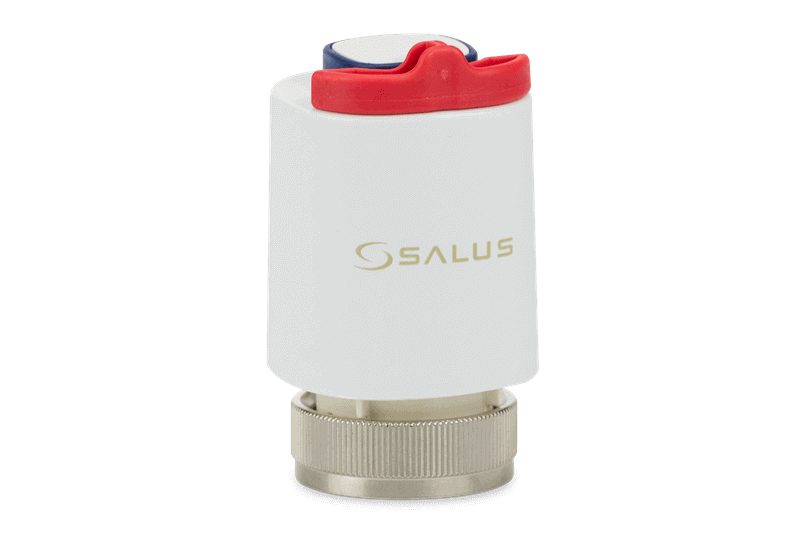
\includegraphics[width=0.8\textwidth]{images/termoelektricky-pohon-salus-t30nc-24-v.png}
    \caption[Termoelektrický pohon Salus T30NC na stejnosměrné napětí 24 V.]{Termoelektrický pohon Salus T30NC na stejnosměrné napětí 24~V \cite{termoelektricky-pohon-t30nc}.}
    \label{fig:termoelektricky-pohon-salus-t30nc-24-v}
\end{figure}

\section{Digitální chodbové termostaty}
\label{digitalni-chodbove-termostaty}
Pro snímání teplot z jednotlivých pater na chodbách slouží digitální termostat s označením W3230. Termostat disponuje jedním spínací výstupem (v případě potřeby vytápění se výstup sepne, jinak je rozepnut). Je možné nastavit hysterezi, časové zpoždění, kalibraci teploty a rozsah maximálních teplot. Lze také aktivovat signalizaci, která se spustí po dosažení maximální přípustné teploty. Pro napájení je potřeba stejnosměrné napětí 12 V. Pro snímání teploty slouží NTC termistor. Rozsah teplot je -40 °C až 120 °C. Přesnost měření je $\pm$ 0,1 °C. Termostat lze nahradit za jakýkoliv jiný, který disponuje spínacím výstupem.


\begin{figure}[H]
    \centering
    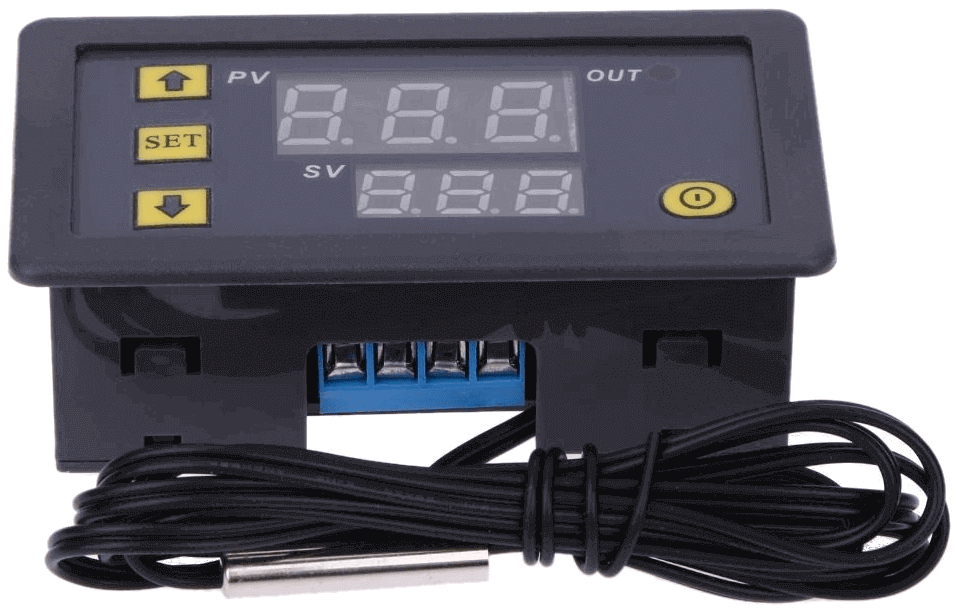
\includegraphics[width=0.8\textwidth]{images/digitalni-termostat-w3230.png}
    \caption[Digitální termostat W3230.]{Digitální termostat W3230 \cite{digitalni-termostat-w3230}.}
    \label{fig:digitalni-termostat-w3230}
\end{figure}


\section{Spínací jednotka}
Pro spínání čerpadel a signalizačních LED slouží dva zakoupené relé moduly po čtyrech kanálech. Relé umožňují spínat výkony 250 VAC při max. 10~A a 30 V DC při max. 10~A. Jednotlivé kanály jsou oddělené galvanicky (dále je vyfrézovaná část DPS mezi výkonovou částí a spínací částí), též je možné využít různých zdrojů pro napájení spínací části a napájení relé. Zapojení jednoho kanálu je obrázku \ref{fig:rele-modul-jeden-kanal}. Celý relé modul je na obrázku \ref{fig:ctyr-kanalovy-rele-modul}.

\begin{figure}[H]
    \centering
    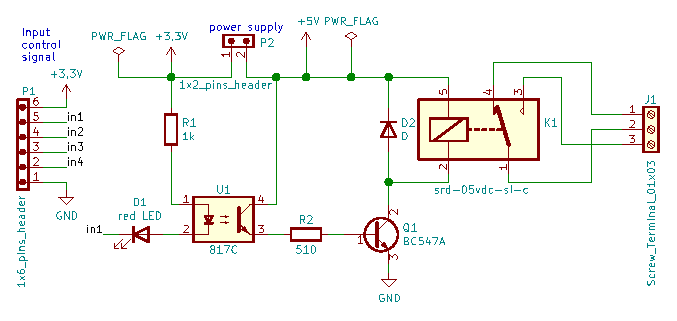
\includegraphics[width=\textwidth]{images/svg/kicad/rele-modul-jeden-kanal.eps}
    \caption{Zapojení jednoho kanálu relé modulu.}
    \label{fig:rele-modul-jeden-kanal}
\end{figure}


\begin{figure}[H]
    \centering
    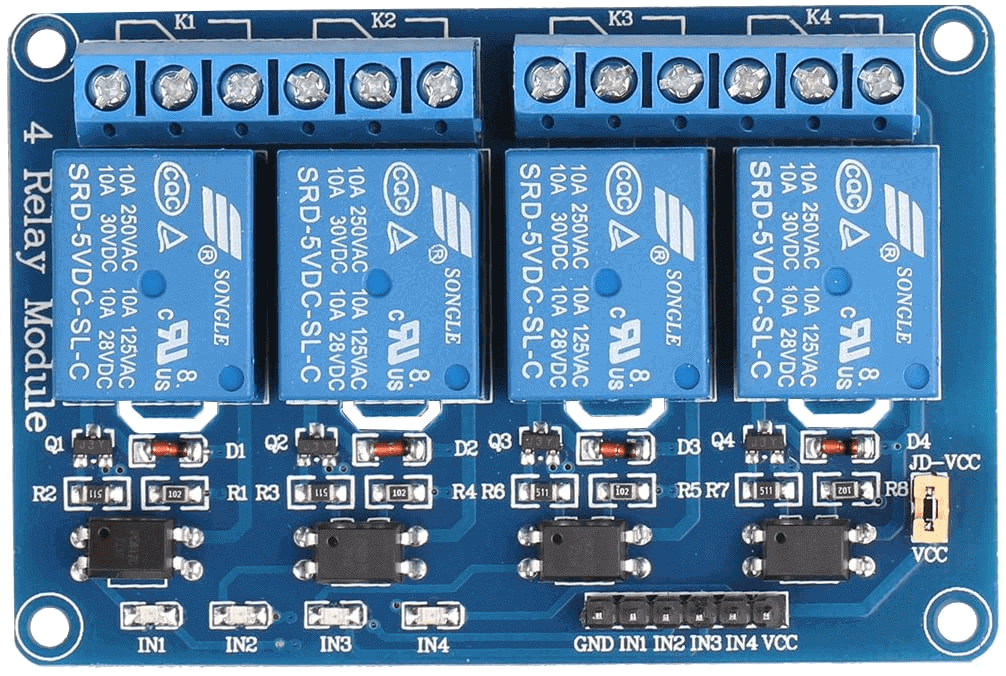
\includegraphics[width=0.8\textwidth]{images/ctyr-kanalovy-rele-modul.png}
    \caption[Čtyř kanálový relé modul.]{Čtyř kanálový relé modul \cite{ctyr-kanalovy-rele-modul}.}
    \label{fig:ctyr-kanalovy-rele-modul}
\end{figure}

\section{Realizovaný rozvaděč s~elektronikou}

V realizovaném rozvaděči na obrázku \ref{fig:rozvadec-ve-sklepe-s-elektronikou} je umístěn 5 V zdroj pro napájení centrální jednotky, relé modulů, I$^2$C diferenciální sběrnice, napájení 1-Wire sběrnice a napájení elektroniky u krbů. Dále je zde 12 V zdroj pro napájení dvou lokálních chodbových termostatů. V  neposlední době jsou zde jističe pro jednotlivé zdroje a čerpadla včetně proudového chrániče.

\newpage

\begin{figure}[H]
    \centering
    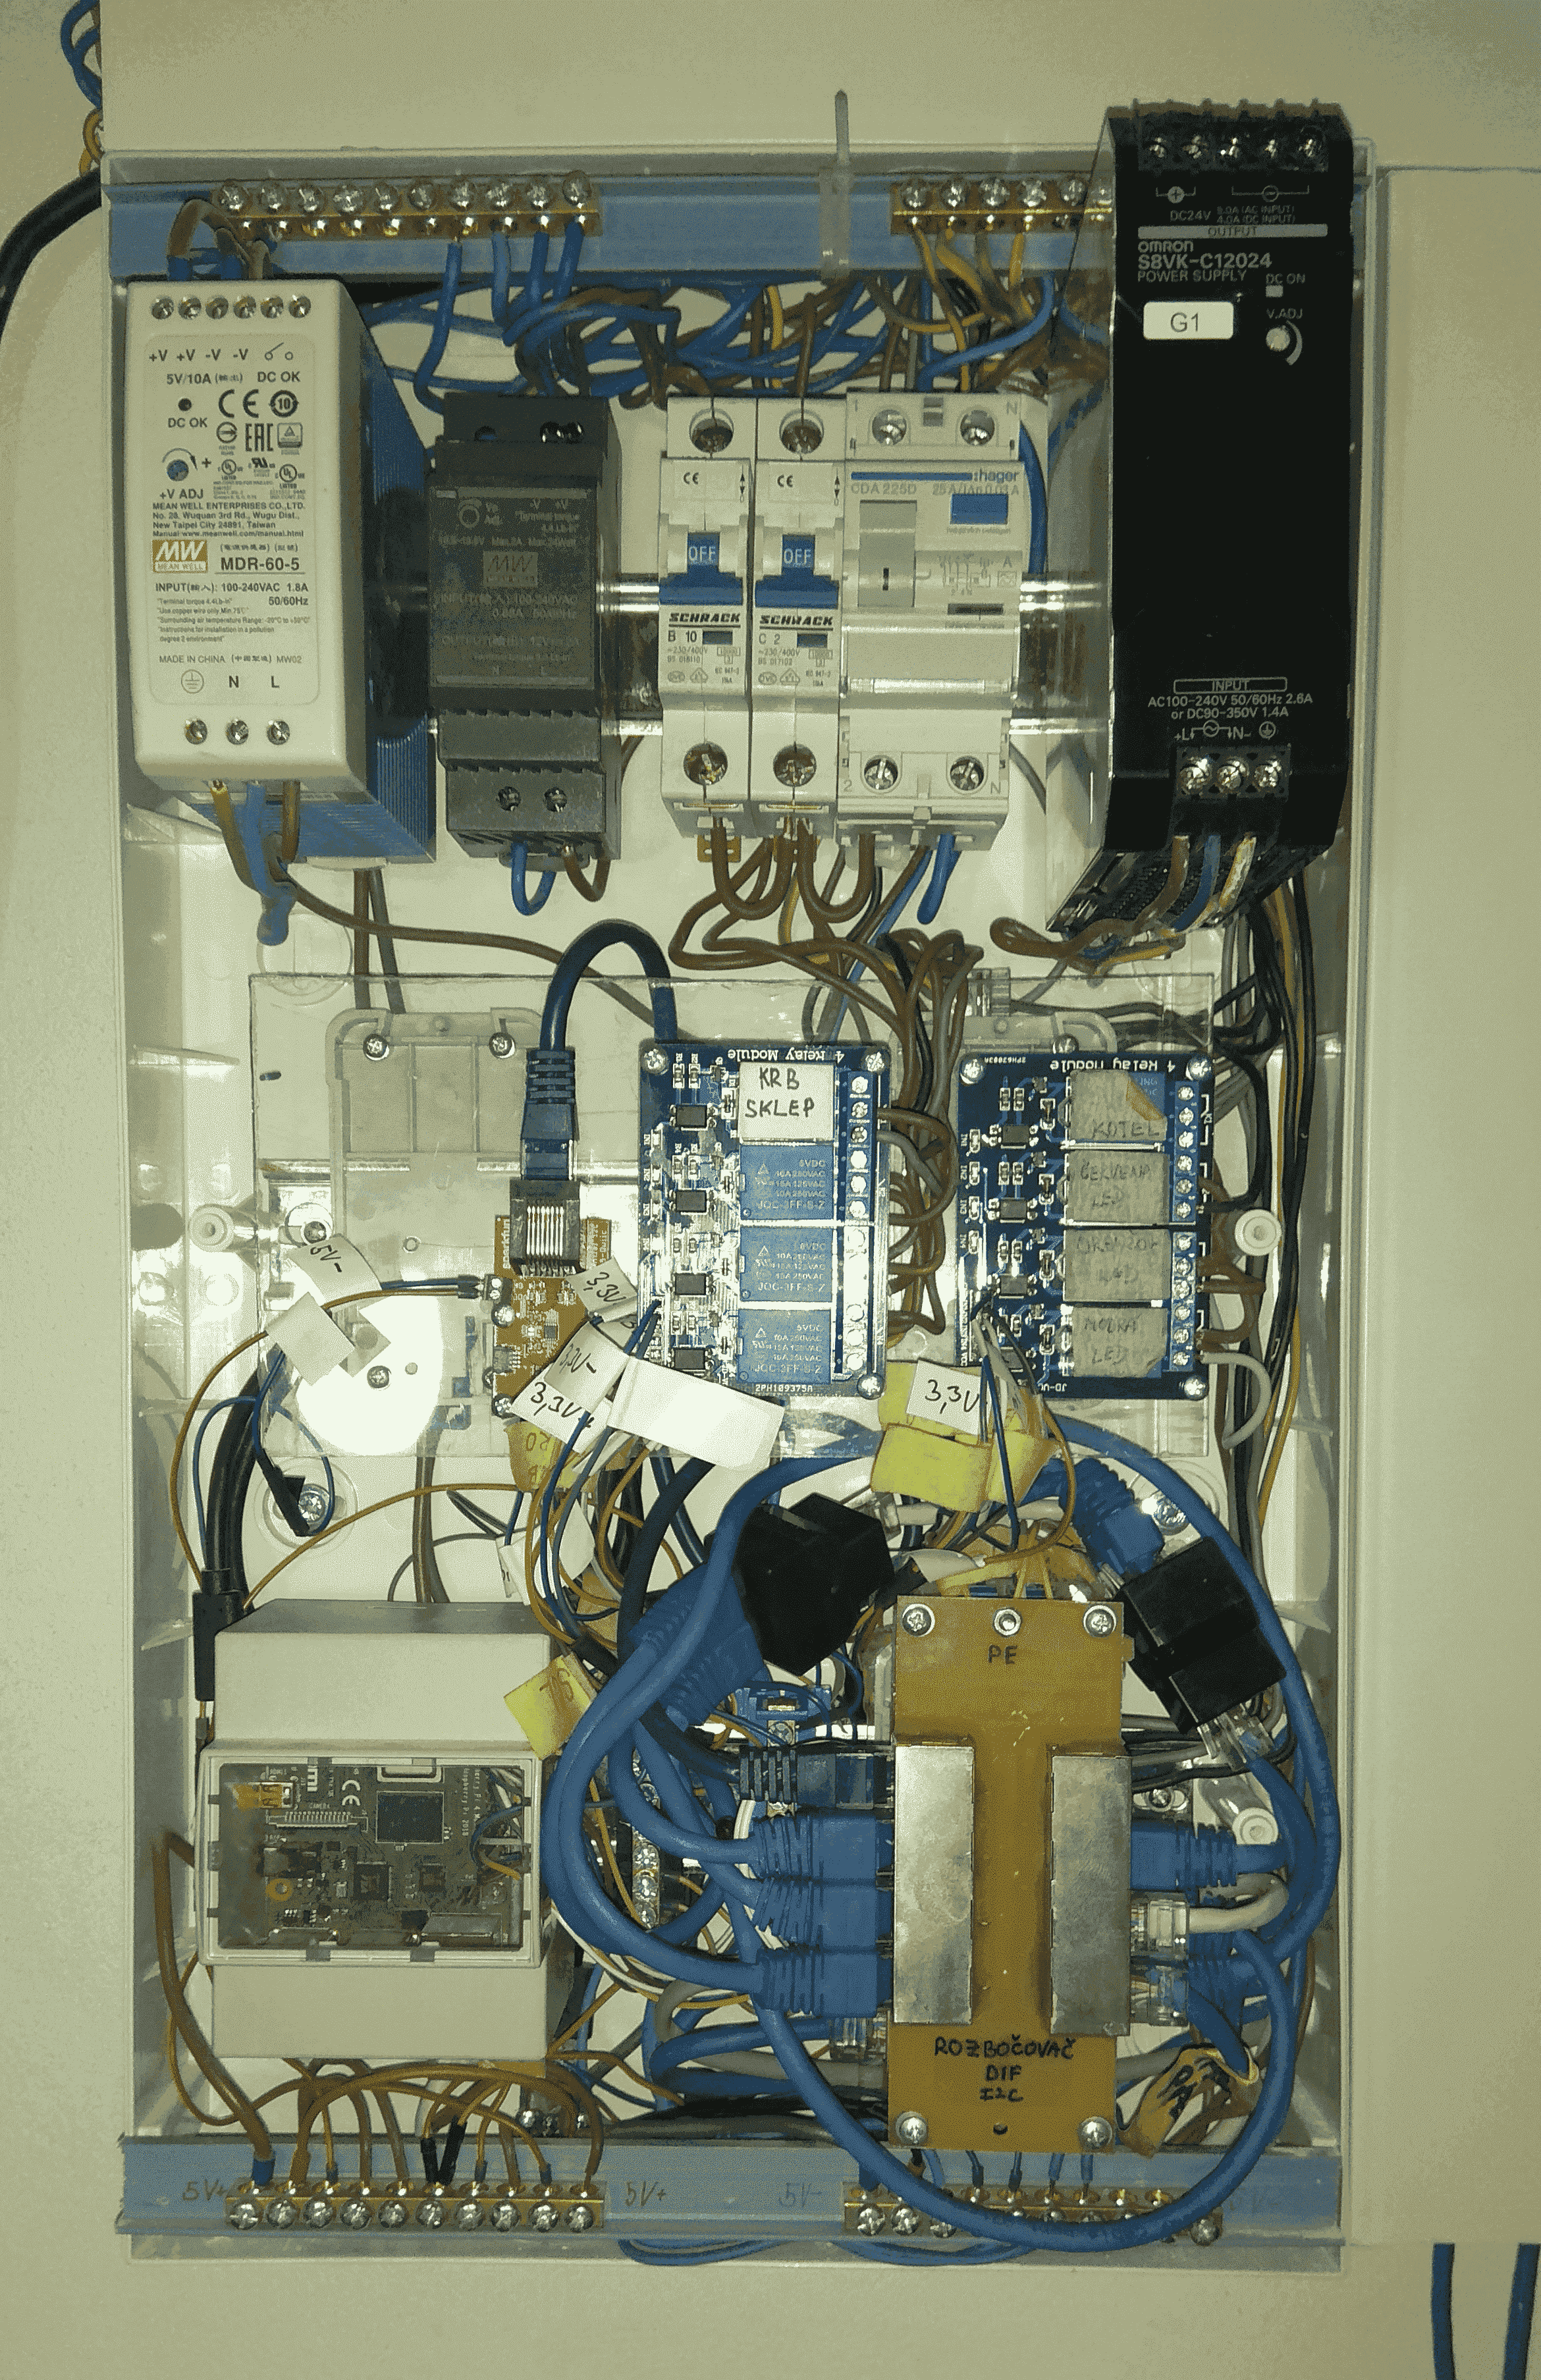
\includegraphics[width=0.99\textwidth]{images/rozvadec-ve-sklepe-s-elektronikou.png}
    \caption{Realizovaný rozvaděč s~elektronikou.}
    \label{fig:rozvadec-ve-sklepe-s-elektronikou}
\end{figure}


\section{Vývoj nástěnného snímače prostorové teploty}
V současné době je ve vývoji nástěnný snímač prostorové teploty. Skládající se z modulu LilyGO TTGO T8 V1.7 s čipem ESP32 obstarávající veškerou obsluhu. Dále z TFT displeje pro zobrazení aktuální naměřené teploty a~požadované teploty. Pro kabelové připojení je zde síťový Ethernet modul W5500. V neposlední řadě je zde teplotní senzor DS18B20 pro měření aktuální teploty v místnosti. Jedná se o prototyp. výsledné zařízení bude uděláno na jednotné DPS s POE napájením.

Modul  LilyGO TTGO T8 V1.7 (obrázek \ref{fig:lilygo-ttgo-v1_7-eps32}) s čipem ESP32, samotný modul obsahuje wifi část, četně miniaturní 3D antény, bluetooth, 4MB Flash, 4MB PSRAM, převodník USB na UART pro programování. Pro zobrazování používám TFT displej (obrázek \ref{fig:predni-cast-tft-lcd-320x240-ili9341}) s rozlišením 320 × 240 px s řadičem ILI9341. Připojení k ESP32 je realizované pomocí SPI sběrnice. Pro  připojení UTP kabelu je použit modul s kontrolérem W5500 pro Ethernet (obrázek~\ref{fig:modul-w5500}), připojení k ESP32 je realizované pomocí SPI sběrnice. 

V současné době nástěnných snímač prostorové teploty snímání okolní teplotu a posílá jí do centrální jednotku, též se zobrazuje na displeji. Nástěnný snímač kontroluje a v případě výpadku se periodicky snaží připojit na centrální jednotku, indikace připojení k centrální jednotce je zobrazena pomocí ikony (zelená ikona WiFi je stav připojeno, červená je stav nepřipojeno). Dále je zde tlačítko pro nastavení požadované teploty, která se dá nastavovat po 0,5 °C, zadaná hodnota se zobrazuje na displeji, též se přenese do centrální jednotky (tam se též zobrazuje pro danou místnost). Každá místnost v patře domu bude osazeno tímto nástěnným snímačem teploty. Místnosti, které jsou bez kabelového připojení. Využívání bezdrátovou komunikační sít WiFi, napájení je pak provedeno přes lokální napájecí adaptér.

\begin{figure}[H]
    \centering
    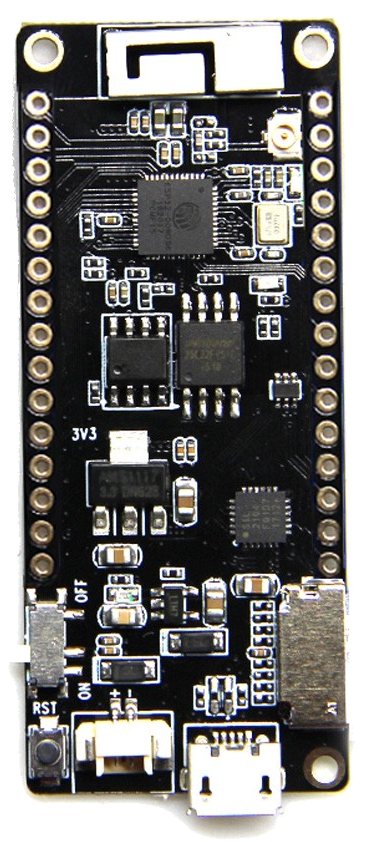
\includegraphics[width=0.3\textwidth]{images/lilygo-ttgo-v1_7-eps32.png}
    \caption[Modul  LilyGO TTGO T8 V1.7.]{Modul  LilyGO TTGO T8 V1.7 \cite{lilygo-ttgo-v1_7-eps32}.}
    \label{fig:lilygo-ttgo-v1_7-eps32}
\end{figure}

\begin{figure}[H]
    \centering
    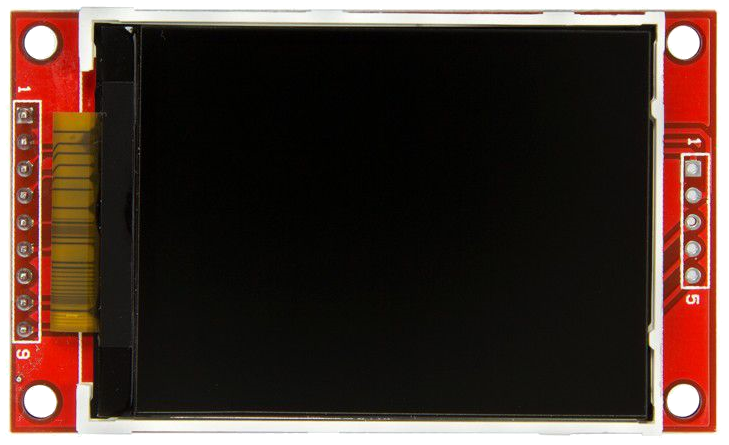
\includegraphics[width=0.6\textwidth]{images/predni-cast-tft-lcd-320x240-ili9341.png}
    \caption[TFT displej s řadičem ILI9341.]{TFT displej s řadičem ILI9341 \cite{tft-lcd-320x240-ili9341}.}
    \label{fig:predni-cast-tft-lcd-320x240-ili9341}
\end{figure}

\begin{figure}[H]
    \centering
    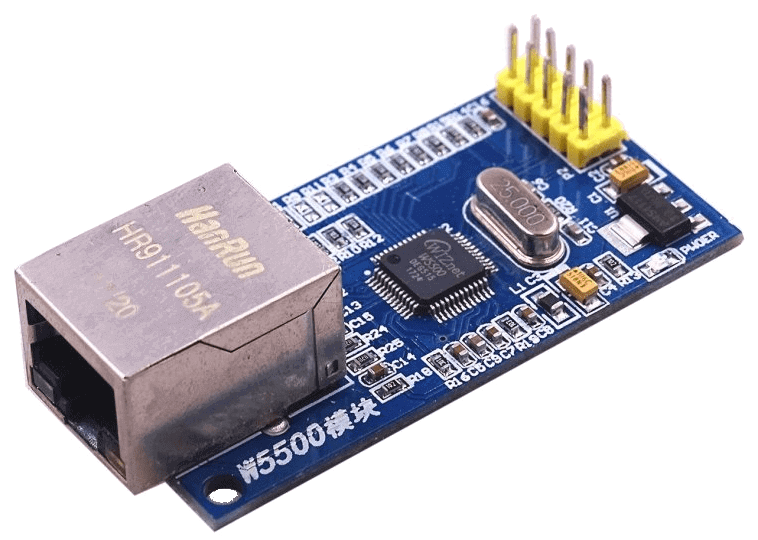
\includegraphics[width=0.6\textwidth]{images/modul-w5500.png}
    \caption[Modul pro připojení Ethernetu.]{Modul pro připojení Ethernetu. \cite{modul-w5500}.}
    \label{fig:modul-w5500}
\end{figure}

\begin{figure}[H]
    \centering
    \includegraphics[width=0.8\textwidth]{images/prototyp-nasteneho-snimace-teploty.png}
    \caption{Zapojení jednotlivých částí přes nepájivé pole.}
    \label{fig:prototyp-nasteneho-snimace-teploty}
\end{figure}

\section{Softwarová část}

\subsection{Záložka nastavení}
V části „módy řízení“ se nachází výběr módů a to zimní, letní nebo výběr podle venkovní teploty. Výběr módu má vliv na výběr mezních teplot pro spínání plynového kondenzačního kotle. Dané teplotní meze se dají nastavit v~části „spínání plynového kotle“ (teplotní meze pro léto a zimu). Tyto nastavené meze se berou pro kontrolu s teplotou v horní části zásobníku otopné vody. Pokud teplota v~horní části zásobníku je menší než teplota definovaná v části „min. zapnutí“ dojde k zapnutí kotle pro nahřátí otopné vody, kotel se vypíná při teplota definované v části „max. vypnutí“. Při porovnávání teplot se též bere v potaz nastavená hystereze v části „ostatní nastavení“. Při výběru módu podle venkovní teploty dochází k automatickému výběru letního nebo zimního módu. Teplotní mez pro výběr letního módu (v rámci módu podle venkovní teploty) je definovaná v části „min. venkovní teplota pro letní mód“. 

V části nastavení „krby – spínání čerpadel“ se definují minimální hranice teploty, kdy dojde k sepnutí oběhových čerpadel pro krbové výměníky, tedy při jaké teplotě se má brát v potaz, zda někdo v krbu zatopit a mají se spustit čerpadla pro nahřívání zásobníku otopné vody. Toto nastavení je poměrně důležité a kontrola těchto teplot je zcela nezávislá na dalších nastaveních (automatizaci) v systému, je potřeba vždy při zatopení spustit čerpadla, jinak dojde k přehřátí vody ve výměníku krbu. V případě přehřátí se aktivuje ochrana přímo u krbů a dojde k ke zvukové signalizaci přehřátí, pokud teplota neklesne za určitou dobu, dojde k aktivování ochranných ventilů a vypuštění přehřáté vody.

V části „LED indikace – mezní parametry zásobníku teplé vody se definují mezní teploty pro horní, střední a spodní část zásobníku otopné vody. Tato signalizace se zejména týká pro krby, aby uživatel věděl, zda může topit a jak je moc zásobník nahřátý. U modré LED se definuje mezní minimální teplota, kterou by zásobníku ve horní části měl mít (povolení pro topení). U oranžové LED se definuje mezní maximální teplota, kdy ve střední části zásobníku dochází k dostatečnému nahřátí otopné vody (oznámení, že za chvilku by se mělo přestat topit). U červené LED se definuje mezní maximální teplota, kdy ve spodní části zásobníku je plně ohřátá(okamžitě přestat topit.). Aktivace červené LED předchází v dostatečném předstihu před aktivováním ochrany u~krbů pro přehřátí otopné vody, popsáno v předchozím odstavci.

Pro přehlednost jsou jednotlivé teploty zobrazeny v části „jednotlivé teploty“, jsou zde všechny teploty snímané v zásobníku otopné vody, teploty na kouřovodech v přízemí a patře, v neposlední řadě jez zde i venkovní teplota. V části „porovnání teploty“ jsou zmíněné teploty zobrazeny v jednom grafu.

Výše popsané části jsou zobrazená na obrázku \ref{fig:ha-nastaveni}.


\begin{figure}[H]
    \centering
    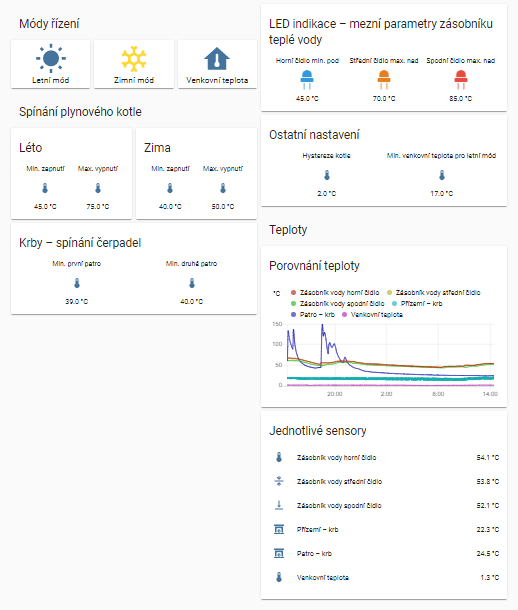
\includegraphics[width=\textwidth]{images/software-ha/ha-nastaveni.png}
    \caption{Záložka nastavení v HA.}
    \label{fig:ha-nastaveni}
\end{figure}

\subsection{Záložka zařízení}
V části „koncová zařízení“ se zobrazují jednotlivá ovládána (zapnuto/vypnuto) zařízení otopné soustavy, tedy plynový kondenzační kotel, čerpadla pro krby s výměníkem, čerpadla pro podlahové vytápění a zapnutí signalizačních LED u krbů. Je možné samotnou automatizaci respektive ovládání zmíněných zařízení řídit podle vlastního uvážení, proto slouží přepínač „manuální ovládání zařízení“, zde si pak uživatel může libovolně jednotlivá zařízení ovládat bez ohledu na nastavenou automatizaci.

V části „termostaty chodby – požadavek topení“, zde se zobrazuje zda dochází k vytápění v přízemí či patře na základě nastavení lokálních termostatů na chodbách.

V části „ovládání čerpadel – vodní kámen“ slouží ke spínání čerpadel pro ochranu před zatuhnutím lopatek. Vzhledem k místní dosti tvrdé vodě, došlo při netopení v přízemí, tedy při nevyužívání daných čerpadel k zatuhnutí lopatek v důsledku nánosu vodního kamene. Pro se zde nachází nastavení, kde si uživatel může pro konkrétní den, hodinu a definovanou délku nastavit spínání čerpadel pro odstranění nánosu na lopatách. Ideální volbou je otopnou vodu zbavit minerálů nebo vyměnit za destilovanou vodu, nicméně k některým méně kvalitnějším provedením spojům trubek otopné soustavy, by docházelo k průsaku otopné vody. Proto je otopná vody z řádu s vyšším podílem minerálů jedním z řešení, jak docílit zaslepení průsaku především vápníkem bez nutnosti, alespoň prozatím, spoje opravovat.

Výše popsané části jsou zobrazená na obrázku \ref{fig:ha-zarizeni}.




\begin{figure}[H]
    \centering
    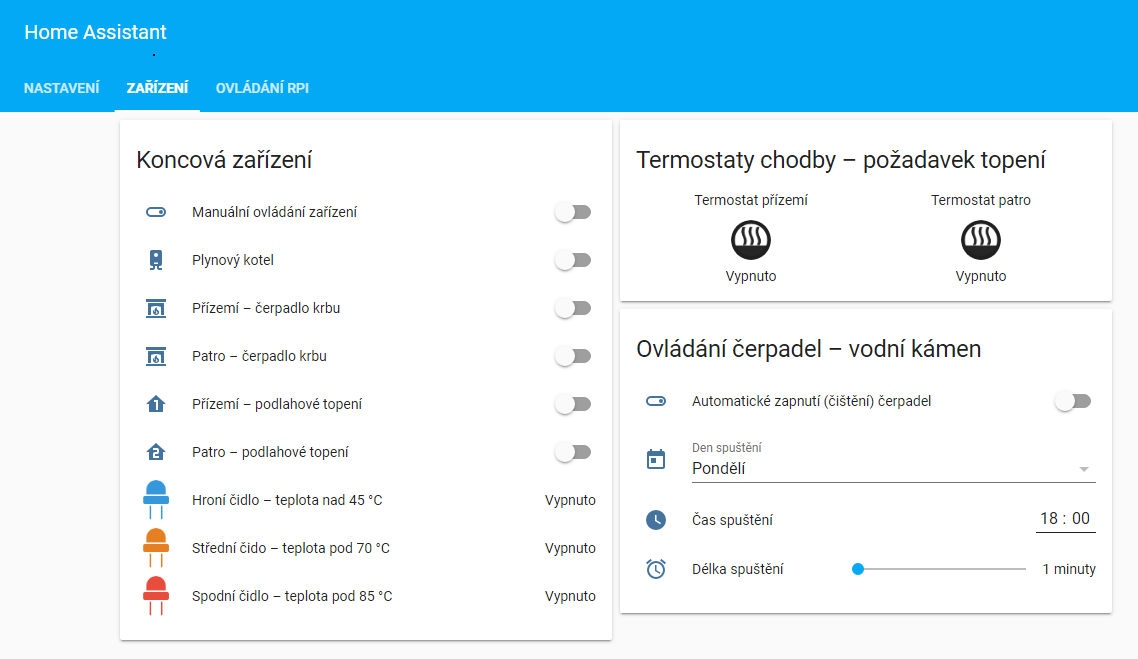
\includegraphics[width=0.90\textwidth]{images/software-ha/ha-zarizeni.png}
    \caption{Záložka zařízení v HA.}
    \label{fig:ha-zarizeni}
\end{figure}

\subsection{Vývoj pro zónovou regulaci}

Na obrázku \ref{fig:teplotni-plan} je zobrazen možný nastavitelný teplotní plán pro celý den. Lze tak nastavit všechny dny v týdnu. Pro každý zvolený teplotní úsek je možné si zvolit požadovanou teplotu.

\begin{figure}[H]
    \centering
    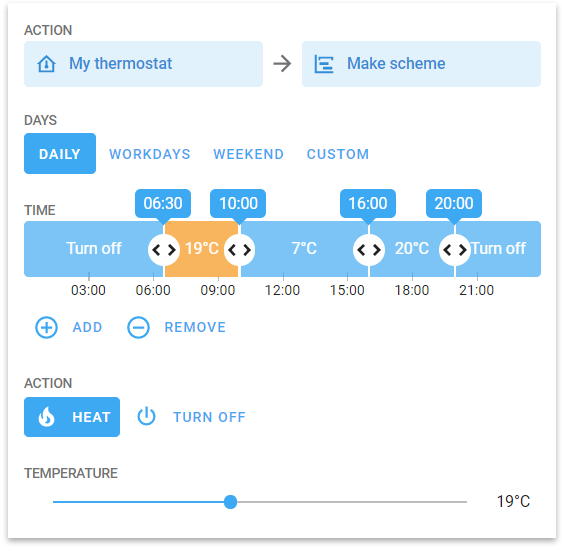
\includegraphics[width=0.90\textwidth]{images/software-ha/teplotni-plan.png}
    \caption{Nastavitelný teplotní plán pro danou hodinu v celém dni.}
    \label{fig:teplotni-plan}
\end{figure}

Na obrázku \ref{fig:termostat-v-mistnosti} je nastavení aktuální teploty pro požadovanou místnost. Každá místnost má svoje vlastní nastavení. Zobrazuje se zde aktuálně naměřená teplota v dané místnosti a požadovaná teplota. Pokud dojde k~přenastavení požadované teploty, dojde k přenesení této teploty do nástěnného snímače prostorové teploty, přenos funguje i opačně.

\begin{figure}[H]
    \centering
    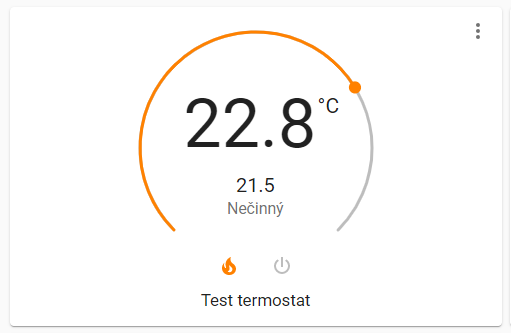
\includegraphics[width=0.90\textwidth]{images/software-ha/termostat-v-mistnosti.png}
    \caption{Zobrazení aktuální teploty z dané místnosti, možnost nastavit požadovanou teplotu.}
    \label{fig:termostat-v-mistnosti}
\end{figure}


